% 2018/11/21

\documentclass[dvipdfmx]{standalone}
% \documentclass[b5paper,papersize,dvipdfmx]{jsarticle}
% \documentclass[b5paper,papersize,dvipdfmx]{jsbook}
%
\usepackage{amsmath}
\usepackage{physics}
\usepackage{here}
\usepackage[dvipdfmx]{graphicx}
% 必須
\usepackage{gnuplot-lua-tikz}
\usepackage{tikz}

\begin{document}
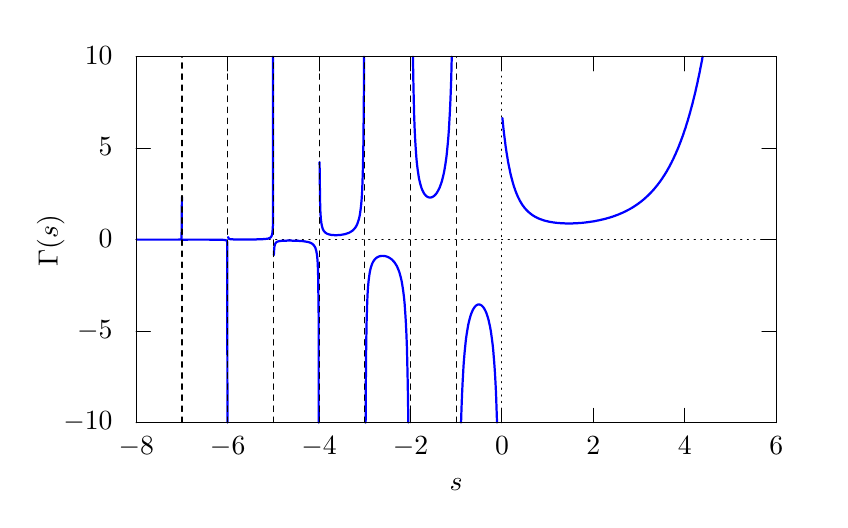
\begin{tikzpicture}[gnuplot]
%% generated with GNUPLOT 5.1p0 (Lua 5.3; terminal rev. 99, script rev. 100)
%% 水 11/21 02:32:06 2018
\path (0.000,0.000) rectangle (10.000,6.000);
\gpcolor{color=gp lt color border}
\gpsetlinetype{gp lt border}
\gpsetdashtype{gp dt solid}
\gpsetlinewidth{1.00}
\draw[gp path] (1.320,0.985)--(1.500,0.985);
\draw[gp path] (9.447,0.985)--(9.267,0.985);
\node[gp node right] at (1.136,0.985) {$-10$};
\draw[gp path] (1.320,2.147)--(1.500,2.147);
\draw[gp path] (9.447,2.147)--(9.267,2.147);
\node[gp node right] at (1.136,2.147) {$-5$};
\draw[gp path] (1.320,3.308)--(1.500,3.308);
\draw[gp path] (9.447,3.308)--(9.267,3.308);
\node[gp node right] at (1.136,3.308) {$0$};
\draw[gp path] (1.320,4.470)--(1.500,4.470);
\draw[gp path] (9.447,4.470)--(9.267,4.470);
\node[gp node right] at (1.136,4.470) {$5$};
\draw[gp path] (1.320,5.631)--(1.500,5.631);
\draw[gp path] (9.447,5.631)--(9.267,5.631);
\node[gp node right] at (1.136,5.631) {$10$};
\draw[gp path] (1.320,0.985)--(1.320,1.165);
\draw[gp path] (1.320,5.631)--(1.320,5.451);
\node[gp node center] at (1.320,0.677) {$-8$};
\draw[gp path] (2.481,0.985)--(2.481,1.165);
\draw[gp path] (2.481,5.631)--(2.481,5.451);
\node[gp node center] at (2.481,0.677) {$-6$};
\draw[gp path] (3.642,0.985)--(3.642,1.165);
\draw[gp path] (3.642,5.631)--(3.642,5.451);
\node[gp node center] at (3.642,0.677) {$-4$};
\draw[gp path] (4.803,0.985)--(4.803,1.165);
\draw[gp path] (4.803,5.631)--(4.803,5.451);
\node[gp node center] at (4.803,0.677) {$-2$};
\draw[gp path] (5.964,0.985)--(5.964,1.165);
\draw[gp path] (5.964,5.631)--(5.964,5.451);
\node[gp node center] at (5.964,0.677) {$0$};
\draw[gp path] (7.125,0.985)--(7.125,1.165);
\draw[gp path] (7.125,5.631)--(7.125,5.451);
\node[gp node center] at (7.125,0.677) {$2$};
\draw[gp path] (8.286,0.985)--(8.286,1.165);
\draw[gp path] (8.286,5.631)--(8.286,5.451);
\node[gp node center] at (8.286,0.677) {$4$};
\draw[gp path] (9.447,0.985)--(9.447,1.165);
\draw[gp path] (9.447,5.631)--(9.447,5.451);
\node[gp node center] at (9.447,0.677) {$6$};
\gpsetlinetype{gp lt axes}
\gpsetdashtype{gp dt axes}
\draw[gp path] (1.320,3.308)--(9.447,3.308);
\draw[gp path] (5.964,0.985)--(5.964,5.631);
\gpsetlinetype{gp lt border}
\gpsetdashtype{gp dt solid}
\draw[gp path] (1.320,5.631)--(1.320,0.985)--(9.447,0.985)--(9.447,5.631)--cycle;
\node[gp node center,rotate=-270] at (0.246,3.308) {$\Gamma(s)$};
\node[gp node center] at (5.383,0.215) {$s$};
\gpcolor{rgb color={0.000,0.000,1.000}}
\gpsetlinewidth{2.00}
\draw[gp path] (8.512,5.631)--(8.507,5.599)--(8.501,5.568)--(8.495,5.538)--(8.489,5.508)%
  --(8.483,5.479)--(8.478,5.449)--(8.472,5.421)--(8.466,5.393)--(8.460,5.365)--(8.454,5.338)%
  --(8.449,5.311)--(8.443,5.284)--(8.437,5.258)--(8.431,5.232)--(8.425,5.207)--(8.420,5.182)%
  --(8.414,5.158)--(8.408,5.134)--(8.402,5.110)--(8.396,5.086)--(8.390,5.063)--(8.385,5.040)%
  --(8.379,5.018)--(8.373,4.996)--(8.367,4.974)--(8.361,4.953)--(8.356,4.932)--(8.350,4.911)%
  --(8.344,4.890)--(8.338,4.870)--(8.332,4.850)--(8.327,4.831)--(8.321,4.812)--(8.315,4.793)%
  --(8.309,4.774)--(8.303,4.755)--(8.298,4.737)--(8.292,4.719)--(8.286,4.702)--(8.280,4.684)%
  --(8.274,4.667)--(8.269,4.650)--(8.263,4.634)--(8.257,4.617)--(8.251,4.601)--(8.245,4.585)%
  --(8.240,4.570)--(8.234,4.554)--(8.228,4.539)--(8.222,4.524)--(8.216,4.509)--(8.211,4.495)%
  --(8.205,4.480)--(8.199,4.466)--(8.193,4.452)--(8.187,4.438)--(8.181,4.425)--(8.176,4.412)%
  --(8.170,4.398)--(8.164,4.385)--(8.158,4.373)--(8.152,4.360)--(8.147,4.348)--(8.141,4.335)%
  --(8.135,4.323)--(8.129,4.311)--(8.123,4.300)--(8.118,4.288)--(8.112,4.277)--(8.106,4.266)%
  --(8.100,4.254)--(8.094,4.244)--(8.089,4.233)--(8.083,4.222)--(8.077,4.212)--(8.071,4.201)%
  --(8.065,4.191)--(8.060,4.181)--(8.054,4.171)--(8.048,4.162)--(8.042,4.152)--(8.036,4.143)%
  --(8.031,4.133)--(8.025,4.124)--(8.019,4.115)--(8.013,4.106)--(8.007,4.097)--(8.002,4.089)%
  --(7.996,4.080)--(7.990,4.072)--(7.984,4.063)--(7.978,4.055)--(7.973,4.047)--(7.967,4.039)%
  --(7.961,4.031)--(7.955,4.023)--(7.949,4.016)--(7.943,4.008)--(7.938,4.000)--(7.932,3.993)%
  --(7.926,3.986)--(7.920,3.979)--(7.914,3.972)--(7.909,3.965)--(7.903,3.958)--(7.897,3.951)%
  --(7.891,3.944)--(7.885,3.938)--(7.880,3.931)--(7.874,3.925)--(7.868,3.919)--(7.862,3.912)%
  --(7.856,3.906)--(7.851,3.900)--(7.845,3.894)--(7.839,3.888)--(7.833,3.882)--(7.827,3.877)%
  --(7.822,3.871)--(7.816,3.865)--(7.810,3.860)--(7.804,3.855)--(7.798,3.849)--(7.793,3.844)%
  --(7.787,3.839)--(7.781,3.834)--(7.775,3.828)--(7.769,3.823)--(7.764,3.818)--(7.758,3.814)%
  --(7.752,3.809)--(7.746,3.804)--(7.740,3.799)--(7.735,3.795)--(7.729,3.790)--(7.723,3.786)%
  --(7.717,3.781)--(7.711,3.777)--(7.705,3.773)--(7.700,3.768)--(7.694,3.764)--(7.688,3.760)%
  --(7.682,3.756)--(7.676,3.752)--(7.671,3.748)--(7.665,3.744)--(7.659,3.740)--(7.653,3.736)%
  --(7.647,3.732)--(7.642,3.729)--(7.636,3.725)--(7.630,3.721)--(7.624,3.718)--(7.618,3.714)%
  --(7.613,3.711)--(7.607,3.707)--(7.601,3.704)--(7.595,3.701)--(7.589,3.697)--(7.584,3.694)%
  --(7.578,3.691)--(7.572,3.688)--(7.566,3.685)--(7.560,3.682)--(7.555,3.679)--(7.549,3.676)%
  --(7.543,3.673)--(7.537,3.670)--(7.531,3.667)--(7.526,3.664)--(7.520,3.661)--(7.514,3.658)%
  --(7.508,3.656)--(7.502,3.653)--(7.497,3.650)--(7.491,3.648)--(7.485,3.645)--(7.479,3.643)%
  --(7.473,3.640)--(7.467,3.638)--(7.462,3.635)--(7.456,3.633)--(7.450,3.630)--(7.444,3.628)%
  --(7.438,3.626)--(7.433,3.623)--(7.427,3.621)--(7.421,3.619)--(7.415,3.617)--(7.409,3.615)%
  --(7.404,3.613)--(7.398,3.610)--(7.392,3.608)--(7.386,3.606)--(7.380,3.604)--(7.375,3.602)%
  --(7.369,3.600)--(7.363,3.598)--(7.357,3.597)--(7.351,3.595)--(7.346,3.593)--(7.340,3.591)%
  --(7.334,3.589)--(7.328,3.587)--(7.322,3.586)--(7.317,3.584)--(7.311,3.582)--(7.305,3.581)%
  --(7.299,3.579)--(7.293,3.577)--(7.288,3.576)--(7.282,3.574)--(7.276,3.573)--(7.270,3.571)%
  --(7.264,3.570)--(7.259,3.568)--(7.253,3.567)--(7.247,3.565)--(7.241,3.564)--(7.235,3.563)%
  --(7.229,3.561)--(7.224,3.560)--(7.218,3.559)--(7.212,3.557)--(7.206,3.556)--(7.200,3.555)%
  --(7.195,3.553)--(7.189,3.552)--(7.183,3.551)--(7.177,3.550)--(7.171,3.549)--(7.166,3.548)%
  --(7.160,3.547)--(7.154,3.545)--(7.148,3.544)--(7.142,3.543)--(7.137,3.542)--(7.131,3.541)%
  --(7.125,3.540)--(7.119,3.539)--(7.113,3.538)--(7.108,3.537)--(7.102,3.537)--(7.096,3.536)%
  --(7.090,3.535)--(7.084,3.534)--(7.079,3.533)--(7.073,3.532)--(7.067,3.531)--(7.061,3.531)%
  --(7.055,3.530)--(7.050,3.529)--(7.044,3.528)--(7.038,3.528)--(7.032,3.527)--(7.026,3.526)%
  --(7.020,3.526)--(7.015,3.525)--(7.009,3.524)--(7.003,3.524)--(6.997,3.523)--(6.991,3.523)%
  --(6.986,3.522)--(6.980,3.521)--(6.974,3.521)--(6.968,3.520)--(6.962,3.520)--(6.957,3.520)%
  --(6.951,3.519)--(6.945,3.519)--(6.939,3.518)--(6.933,3.518)--(6.928,3.517)--(6.922,3.517)%
  --(6.916,3.517)--(6.910,3.516)--(6.904,3.516)--(6.899,3.516)--(6.893,3.516)--(6.887,3.515)%
  --(6.881,3.515)--(6.875,3.515)--(6.870,3.515)--(6.864,3.514)--(6.858,3.514)--(6.852,3.514)%
  --(6.846,3.514)--(6.841,3.514)--(6.835,3.514)--(6.829,3.514)--(6.823,3.514)--(6.817,3.514)%
  --(6.812,3.514)--(6.806,3.514)--(6.800,3.514)--(6.794,3.514)--(6.788,3.514)--(6.782,3.514)%
  --(6.777,3.514)--(6.771,3.514)--(6.765,3.514)--(6.759,3.515)--(6.753,3.515)--(6.748,3.515)%
  --(6.742,3.515)--(6.736,3.516)--(6.730,3.516)--(6.724,3.516)--(6.719,3.516)--(6.713,3.517)%
  --(6.707,3.517)--(6.701,3.518)--(6.695,3.518)--(6.690,3.519)--(6.684,3.519)--(6.678,3.520)%
  --(6.672,3.520)--(6.666,3.521)--(6.661,3.521)--(6.655,3.522)--(6.649,3.523)--(6.643,3.523)%
  --(6.637,3.524)--(6.632,3.525)--(6.626,3.525)--(6.620,3.526)--(6.614,3.527)--(6.608,3.528)%
  --(6.603,3.529)--(6.597,3.530)--(6.591,3.531)--(6.585,3.532)--(6.579,3.533)--(6.574,3.534)%
  --(6.568,3.535)--(6.562,3.536)--(6.556,3.538)--(6.550,3.539)--(6.544,3.540)--(6.539,3.542)%
  --(6.533,3.543)--(6.527,3.544)--(6.521,3.546)--(6.515,3.547)--(6.510,3.549)--(6.504,3.551)%
  --(6.498,3.552)--(6.492,3.554)--(6.486,3.556)--(6.481,3.558)--(6.475,3.560)--(6.469,3.562)%
  --(6.463,3.564)--(6.457,3.566)--(6.452,3.568)--(6.446,3.570)--(6.440,3.573)--(6.434,3.575)%
  --(6.428,3.578)--(6.423,3.580)--(6.417,3.583)--(6.411,3.586)--(6.405,3.589)--(6.399,3.592)%
  --(6.394,3.595)--(6.388,3.598)--(6.382,3.601)--(6.376,3.604)--(6.370,3.608)--(6.365,3.611)%
  --(6.359,3.615)--(6.353,3.619)--(6.347,3.623)--(6.341,3.627)--(6.336,3.631)--(6.330,3.636)%
  --(6.324,3.640)--(6.318,3.645)--(6.312,3.650)--(6.306,3.655)--(6.301,3.660)--(6.295,3.665)%
  --(6.289,3.671)--(6.283,3.677)--(6.277,3.683)--(6.272,3.689)--(6.266,3.695)--(6.260,3.702)%
  --(6.254,3.709)--(6.248,3.716)--(6.243,3.724)--(6.237,3.731)--(6.231,3.739)--(6.225,3.748)%
  --(6.219,3.756)--(6.214,3.765)--(6.208,3.775)--(6.202,3.785)--(6.196,3.795)--(6.190,3.805)%
  --(6.185,3.816)--(6.179,3.828)--(6.173,3.839)--(6.167,3.852)--(6.161,3.865)--(6.156,3.878)%
  --(6.150,3.892)--(6.144,3.907)--(6.138,3.922)--(6.132,3.938)--(6.127,3.954)--(6.121,3.971)%
  --(6.115,3.989)--(6.109,4.008)--(6.103,4.028)--(6.098,4.048)--(6.092,4.070)--(6.086,4.092)%
  --(6.080,4.116)--(6.074,4.140)--(6.068,4.166)--(6.063,4.193)--(6.057,4.221)--(6.051,4.250)%
  --(6.045,4.281)--(6.039,4.313)--(6.034,4.347)--(6.028,4.383)--(6.022,4.420)--(6.016,4.459)%
  --(6.010,4.500)--(6.005,4.543)--(5.999,4.589)--(5.993,4.636)--(5.987,4.686)--(5.981,4.739)%
  --(5.976,4.794)--(5.970,4.852);
\draw[gp path] (5.901,0.985)--(5.900,1.034)--(5.894,1.207)--(5.889,1.353)--(5.883,1.477)%
  --(5.877,1.585)--(5.871,1.679)--(5.865,1.761)--(5.859,1.833)--(5.854,1.898)--(5.848,1.956)%
  --(5.842,2.007)--(5.836,2.054)--(5.830,2.096)--(5.825,2.135)--(5.819,2.169)--(5.813,2.201)%
  --(5.807,2.230)--(5.801,2.256)--(5.796,2.281)--(5.790,2.303)--(5.784,2.323)--(5.778,2.342)%
  --(5.772,2.359)--(5.767,2.375)--(5.761,2.389)--(5.755,2.402)--(5.749,2.414)--(5.743,2.425)%
  --(5.738,2.434)--(5.732,2.443)--(5.726,2.451)--(5.720,2.458)--(5.714,2.464)--(5.709,2.469)%
  --(5.703,2.474)--(5.697,2.477)--(5.691,2.480)--(5.685,2.482)--(5.680,2.484)--(5.674,2.484)%
  --(5.668,2.484)--(5.662,2.484)--(5.656,2.482)--(5.651,2.480)--(5.645,2.477)--(5.639,2.473)%
  --(5.633,2.468)--(5.627,2.463)--(5.621,2.456)--(5.616,2.449)--(5.610,2.441)--(5.604,2.432)%
  --(5.598,2.422)--(5.592,2.410)--(5.587,2.398)--(5.581,2.384)--(5.575,2.369)--(5.569,2.353)%
  --(5.563,2.335)--(5.558,2.315)--(5.552,2.294)--(5.546,2.270)--(5.540,2.244)--(5.534,2.216)%
  --(5.529,2.185)--(5.523,2.151)--(5.517,2.113)--(5.511,2.072)--(5.505,2.026)--(5.500,1.975)%
  --(5.494,1.918)--(5.488,1.854)--(5.482,1.782)--(5.476,1.701)--(5.471,1.608)--(5.465,1.501)%
  --(5.459,1.377)--(5.453,1.232)--(5.447,1.060)--(5.445,0.985);
\draw[gp path] (5.327,5.631)--(5.325,5.564)--(5.320,5.356)--(5.314,5.184)--(5.308,5.038)%
  --(5.302,4.913)--(5.296,4.806)--(5.291,4.712)--(5.285,4.630)--(5.279,4.557)--(5.273,4.493)%
  --(5.267,4.435)--(5.262,4.383)--(5.256,4.336)--(5.250,4.293)--(5.244,4.254)--(5.238,4.219)%
  --(5.233,4.187)--(5.227,4.157)--(5.221,4.130)--(5.215,4.104)--(5.209,4.081)--(5.204,4.060)%
  --(5.198,4.040)--(5.192,4.022)--(5.186,4.005)--(5.180,3.989)--(5.175,3.974)--(5.169,3.961)%
  --(5.163,3.948)--(5.157,3.937)--(5.151,3.926)--(5.145,3.916)--(5.140,3.907)--(5.134,3.898)%
  --(5.128,3.890)--(5.122,3.883)--(5.116,3.877)--(5.111,3.871)--(5.105,3.866)--(5.099,3.861)%
  --(5.093,3.857)--(5.087,3.853)--(5.082,3.850)--(5.076,3.848)--(5.070,3.846)--(5.064,3.844)%
  --(5.058,3.843)--(5.053,3.843)--(5.047,3.843)--(5.041,3.844)--(5.035,3.845)--(5.029,3.847)%
  --(5.024,3.849)--(5.018,3.852)--(5.012,3.855)--(5.006,3.860)--(5.000,3.864)--(4.995,3.870)%
  --(4.989,3.877)--(4.983,3.884)--(4.977,3.892)--(4.971,3.901)--(4.966,3.911)--(4.960,3.923)%
  --(4.954,3.936)--(4.948,3.950)--(4.942,3.965)--(4.937,3.983)--(4.931,4.002)--(4.925,4.024)%
  --(4.919,4.049)--(4.913,4.076)--(4.907,4.107)--(4.902,4.142)--(4.896,4.182)--(4.890,4.227)%
  --(4.884,4.279)--(4.878,4.341)--(4.873,4.412)--(4.867,4.498)--(4.861,4.601)--(4.855,4.727)%
  --(4.849,4.886)--(4.844,5.091)--(4.838,5.365)--(4.834,5.631);
\draw[gp path] (4.775,0.985)--(4.774,1.082)--(4.768,1.467)--(4.762,1.742)--(4.757,1.947)%
  --(4.751,2.106)--(4.745,2.234)--(4.739,2.337)--(4.733,2.423)--(4.728,2.496)--(4.722,2.558)%
  --(4.716,2.611)--(4.710,2.658)--(4.704,2.699)--(4.698,2.735)--(4.693,2.767)--(4.687,2.796)%
  --(4.681,2.822)--(4.675,2.845)--(4.669,2.866)--(4.664,2.886)--(4.658,2.903)--(4.652,2.919)%
  --(4.646,2.934)--(4.640,2.948)--(4.635,2.960)--(4.629,2.972)--(4.623,2.983)--(4.617,2.993)%
  --(4.611,3.002)--(4.606,3.010)--(4.600,3.018)--(4.594,3.026)--(4.588,3.033)--(4.582,3.039)%
  --(4.577,3.045)--(4.571,3.051)--(4.565,3.056)--(4.559,3.061)--(4.553,3.065)--(4.548,3.069)%
  --(4.542,3.073)--(4.536,3.077)--(4.530,3.080)--(4.524,3.083)--(4.519,3.086)--(4.513,3.088)%
  --(4.507,3.091)--(4.501,3.093)--(4.495,3.095)--(4.490,3.096)--(4.484,3.098)--(4.478,3.099)%
  --(4.472,3.100)--(4.466,3.101)--(4.460,3.101)--(4.455,3.102)--(4.449,3.102)--(4.443,3.102)%
  --(4.437,3.101)--(4.431,3.101)--(4.426,3.100)--(4.420,3.099)--(4.414,3.097)--(4.408,3.096)%
  --(4.402,3.094)--(4.397,3.092)--(4.391,3.089)--(4.385,3.086)--(4.379,3.083)--(4.373,3.079)%
  --(4.368,3.075)--(4.362,3.070)--(4.356,3.064)--(4.350,3.058)--(4.344,3.051)--(4.339,3.043)%
  --(4.333,3.035)--(4.327,3.025)--(4.321,3.013)--(4.315,3.000)--(4.310,2.986)--(4.304,2.968)%
  --(4.298,2.948)--(4.292,2.925)--(4.286,2.896)--(4.281,2.862)--(4.275,2.820)--(4.269,2.768)%
  --(4.263,2.699)--(4.257,2.608)--(4.252,2.480)--(4.246,2.287)--(4.240,1.965)--(4.234,1.320)%
  --(4.233,0.985);
\draw[gp path] (4.212,5.631)--(4.211,5.195)--(4.205,4.552)--(4.199,4.230)--(4.193,4.038)%
  --(4.188,3.910)--(4.182,3.818)--(4.176,3.750)--(4.170,3.697)--(4.164,3.655)--(4.159,3.620)%
  --(4.153,3.592)--(4.147,3.567)--(4.141,3.547)--(4.135,3.529)--(4.130,3.514)--(4.124,3.500)%
  --(4.118,3.488)--(4.112,3.478)--(4.106,3.468)--(4.101,3.459)--(4.095,3.452)--(4.089,3.445)%
  --(4.083,3.438)--(4.077,3.433)--(4.072,3.427)--(4.066,3.422)--(4.060,3.418)--(4.054,3.414)%
  --(4.048,3.410)--(4.043,3.406)--(4.037,3.403)--(4.031,3.400)--(4.025,3.397)--(4.019,3.394)%
  --(4.014,3.392)--(4.008,3.390)--(4.002,3.388)--(3.996,3.386)--(3.990,3.384)--(3.984,3.382)%
  --(3.979,3.380)--(3.973,3.379)--(3.967,3.377)--(3.961,3.376)--(3.955,3.375)--(3.950,3.374)%
  --(3.944,3.373)--(3.938,3.372)--(3.932,3.371)--(3.926,3.370)--(3.921,3.369)--(3.915,3.368)%
  --(3.909,3.368)--(3.903,3.367)--(3.897,3.367)--(3.892,3.366)--(3.886,3.366)--(3.880,3.366)%
  --(3.874,3.365)--(3.868,3.365)--(3.863,3.365)--(3.857,3.365)--(3.851,3.365)--(3.845,3.365)%
  --(3.839,3.365)--(3.834,3.365)--(3.828,3.366)--(3.822,3.366)--(3.816,3.366)--(3.810,3.367)%
  --(3.805,3.368)--(3.799,3.368)--(3.793,3.369)--(3.787,3.370)--(3.781,3.371)--(3.776,3.373)%
  --(3.770,3.374)--(3.764,3.376)--(3.758,3.378)--(3.752,3.380)--(3.746,3.382)--(3.741,3.385)%
  --(3.735,3.388)--(3.729,3.392)--(3.723,3.396)--(3.717,3.401)--(3.712,3.407)--(3.706,3.414)%
  --(3.700,3.422)--(3.694,3.433)--(3.688,3.446)--(3.683,3.463)--(3.677,3.486)--(3.671,3.518)%
  --(3.665,3.566)--(3.659,3.646)--(3.654,3.807)--(3.648,4.292);
\draw[gp path] (3.636,0.985)--(3.636,2.356)--(3.630,2.838)--(3.625,2.999)--(3.619,3.080)%
  --(3.613,3.128)--(3.607,3.160)--(3.601,3.183)--(3.596,3.200)--(3.590,3.213)--(3.584,3.223)%
  --(3.578,3.232)--(3.572,3.239)--(3.567,3.245)--(3.561,3.250)--(3.555,3.255)--(3.549,3.259)%
  --(3.543,3.262)--(3.537,3.265)--(3.532,3.268)--(3.526,3.270)--(3.520,3.272)--(3.514,3.274)%
  --(3.508,3.276)--(3.503,3.277)--(3.497,3.279)--(3.491,3.280)--(3.485,3.281)--(3.479,3.282)%
  --(3.474,3.283)--(3.468,3.284)--(3.462,3.285)--(3.456,3.286)--(3.450,3.287)--(3.445,3.287)%
  --(3.439,3.288)--(3.433,3.289)--(3.427,3.289)--(3.421,3.290)--(3.416,3.290)--(3.410,3.291)%
  --(3.404,3.291)--(3.398,3.292)--(3.392,3.292)--(3.387,3.292)--(3.381,3.293)--(3.375,3.293)%
  --(3.369,3.293)--(3.363,3.294)--(3.358,3.294)--(3.352,3.294)--(3.346,3.294)--(3.340,3.294)%
  --(3.334,3.295)--(3.329,3.295)--(3.323,3.295)--(3.317,3.295)--(3.311,3.295)--(3.305,3.295)%
  --(3.299,3.295)--(3.294,3.296)--(3.288,3.296)--(3.282,3.296)--(3.276,3.296)--(3.270,3.296)%
  --(3.265,3.296)--(3.259,3.296)--(3.253,3.296)--(3.247,3.296)--(3.241,3.296)--(3.236,3.296)%
  --(3.230,3.295)--(3.224,3.295)--(3.218,3.295)--(3.212,3.295)--(3.207,3.295)--(3.201,3.295)%
  --(3.195,3.294)--(3.189,3.294)--(3.183,3.294)--(3.178,3.293)--(3.172,3.293)--(3.166,3.293)%
  --(3.160,3.292)--(3.154,3.291)--(3.149,3.291)--(3.143,3.290)--(3.137,3.289)--(3.131,3.288)%
  --(3.125,3.286)--(3.120,3.285)--(3.114,3.283)--(3.108,3.280)--(3.102,3.277)--(3.096,3.272)%
  --(3.091,3.266)--(3.085,3.256)--(3.079,3.240)--(3.073,3.208)--(3.067,3.110);
\draw[gp path] (3.056,5.631)--(3.056,3.498)--(3.050,3.401)--(3.044,3.369)--(3.038,3.353)%
  --(3.032,3.344)--(3.027,3.337)--(3.021,3.333)--(3.015,3.329)--(3.009,3.327)--(3.003,3.325)%
  --(2.998,3.323)--(2.992,3.321)--(2.986,3.320)--(2.980,3.319)--(2.974,3.318)--(2.969,3.318)%
  --(2.963,3.317)--(2.957,3.316)--(2.951,3.316)--(2.945,3.315)--(2.940,3.315)--(2.934,3.315)%
  --(2.928,3.314)--(2.922,3.314)--(2.916,3.314)--(2.911,3.313)--(2.905,3.313)--(2.899,3.313)%
  --(2.893,3.313)--(2.887,3.312)--(2.882,3.312)--(2.876,3.312)--(2.870,3.312)--(2.864,3.312)%
  --(2.858,3.312)--(2.852,3.312)--(2.847,3.311)--(2.841,3.311)--(2.835,3.311)--(2.829,3.311)%
  --(2.823,3.311)--(2.818,3.311)--(2.812,3.311)--(2.806,3.311)--(2.800,3.311)--(2.794,3.311)%
  --(2.789,3.311)--(2.783,3.311)--(2.777,3.311)--(2.771,3.311)--(2.765,3.310)--(2.760,3.310)%
  --(2.754,3.310)--(2.748,3.310)--(2.742,3.310)--(2.736,3.310)--(2.731,3.310)--(2.725,3.310)%
  --(2.719,3.310)--(2.713,3.310)--(2.707,3.310)--(2.702,3.310)--(2.696,3.310)--(2.690,3.310)%
  --(2.684,3.310)--(2.678,3.310)--(2.673,3.310)--(2.667,3.310)--(2.661,3.310)--(2.655,3.310)%
  --(2.649,3.310)--(2.644,3.310)--(2.638,3.310)--(2.632,3.310)--(2.626,3.310)--(2.620,3.310)%
  --(2.614,3.310)--(2.609,3.310)--(2.603,3.310)--(2.597,3.311)--(2.591,3.311)--(2.585,3.311)%
  --(2.580,3.311)--(2.574,3.311)--(2.568,3.311)--(2.562,3.311)--(2.556,3.311)--(2.551,3.311)%
  --(2.545,3.312)--(2.539,3.312)--(2.533,3.312)--(2.527,3.313)--(2.522,3.313)--(2.516,3.314)%
  --(2.510,3.315)--(2.504,3.317)--(2.498,3.319)--(2.493,3.325)--(2.487,3.341);
\draw[gp path] (2.478,0.985)--(2.475,3.277)--(2.469,3.293)--(2.464,3.298)--(2.458,3.301)%
  --(2.452,3.302)--(2.446,3.303)--(2.440,3.304)--(2.435,3.304)--(2.429,3.305)--(2.423,3.305)%
  --(2.417,3.306)--(2.411,3.306)--(2.405,3.306)--(2.400,3.306)--(2.394,3.306)--(2.388,3.306)%
  --(2.382,3.307)--(2.376,3.307)--(2.371,3.307)--(2.365,3.307)--(2.359,3.307)--(2.353,3.307)%
  --(2.347,3.307)--(2.342,3.307)--(2.336,3.307)--(2.330,3.307)--(2.324,3.307)--(2.318,3.307)%
  --(2.313,3.307)--(2.307,3.307)--(2.301,3.307)--(2.295,3.307)--(2.289,3.307)--(2.284,3.307)%
  --(2.278,3.307)--(2.272,3.307)--(2.266,3.307)--(2.260,3.307)--(2.255,3.307)--(2.249,3.308)%
  --(2.243,3.308)--(2.237,3.308)--(2.231,3.308)--(2.226,3.308)--(2.220,3.308)--(2.214,3.308)%
  --(2.208,3.308)--(2.202,3.308)--(2.197,3.308)--(2.191,3.308)--(2.185,3.308)--(2.179,3.308)%
  --(2.173,3.308)--(2.167,3.308)--(2.162,3.308)--(2.156,3.308)--(2.150,3.308)--(2.144,3.308)%
  --(2.138,3.308)--(2.133,3.308)--(2.127,3.308)--(2.121,3.308)--(2.115,3.308)--(2.109,3.308)%
  --(2.104,3.308)--(2.098,3.308)--(2.092,3.308)--(2.086,3.308)--(2.080,3.308)--(2.075,3.308)%
  --(2.069,3.308)--(2.063,3.308)--(2.057,3.308)--(2.051,3.308)--(2.046,3.308)--(2.040,3.308)%
  --(2.034,3.308)--(2.028,3.308)--(2.022,3.308)--(2.017,3.308)--(2.011,3.308)--(2.005,3.308)%
  --(1.999,3.308)--(1.993,3.308)--(1.988,3.308)--(1.982,3.308)--(1.976,3.308)--(1.970,3.307)%
  --(1.964,3.307)--(1.959,3.307)--(1.953,3.307)--(1.947,3.307)--(1.941,3.307)--(1.935,3.307)%
  --(1.929,3.307)--(1.924,3.307)--(1.918,3.306)--(1.912,3.306)--(1.906,3.303);
\draw[gp path] (1.900,3.853)--(1.895,3.312)--(1.889,3.310)--(1.883,3.309)--(1.877,3.309)%
  --(1.871,3.309)--(1.866,3.309)--(1.860,3.309)--(1.854,3.308)--(1.848,3.308)--(1.842,3.308)%
  --(1.837,3.308)--(1.831,3.308)--(1.825,3.308)--(1.819,3.308)--(1.813,3.308)--(1.808,3.308)%
  --(1.802,3.308)--(1.796,3.308)--(1.790,3.308)--(1.784,3.308)--(1.779,3.308)--(1.773,3.308)%
  --(1.767,3.308)--(1.761,3.308)--(1.755,3.308)--(1.750,3.308)--(1.744,3.308)--(1.738,3.308)%
  --(1.732,3.308)--(1.726,3.308)--(1.720,3.308)--(1.715,3.308)--(1.709,3.308)--(1.703,3.308)%
  --(1.697,3.308)--(1.691,3.308)--(1.686,3.308)--(1.680,3.308)--(1.674,3.308)--(1.668,3.308)%
  --(1.662,3.308)--(1.657,3.308)--(1.651,3.308)--(1.645,3.308)--(1.639,3.308)--(1.633,3.308)%
  --(1.628,3.308)--(1.622,3.308)--(1.616,3.308)--(1.610,3.308)--(1.604,3.308)--(1.599,3.308)%
  --(1.593,3.308)--(1.587,3.308)--(1.581,3.308)--(1.575,3.308)--(1.570,3.308)--(1.564,3.308)%
  --(1.558,3.308)--(1.552,3.308)--(1.546,3.308)--(1.541,3.308)--(1.535,3.308)--(1.529,3.308)%
  --(1.523,3.308)--(1.517,3.308)--(1.512,3.308)--(1.506,3.308)--(1.500,3.308)--(1.494,3.308)%
  --(1.488,3.308)--(1.482,3.308)--(1.477,3.308)--(1.471,3.308)--(1.465,3.308)--(1.459,3.308)%
  --(1.453,3.308)--(1.448,3.308)--(1.442,3.308)--(1.436,3.308)--(1.430,3.308)--(1.424,3.308)%
  --(1.419,3.308)--(1.413,3.308)--(1.407,3.308)--(1.401,3.308)--(1.395,3.308)--(1.390,3.308)%
  --(1.384,3.308)--(1.378,3.308)--(1.372,3.308)--(1.366,3.308)--(1.361,3.308)--(1.355,3.308)%
  --(1.349,3.308)--(1.343,3.308)--(1.337,3.308)--(1.332,3.308)--(1.326,3.309);
\gpcolor{rgb color={0.000,0.000,0.000}}
\gpsetdashtype{dash pattern=on 5.00*\gpdashlength off 5.00*\gpdashlength }
\gpsetlinewidth{1.00}
\draw[gp path] (5.384,0.985)--(5.384,1.032)--(5.384,1.079)--(5.384,1.126)--(5.384,1.173)%
  --(5.384,1.220)--(5.384,1.267)--(5.384,1.314)--(5.384,1.360)--(5.384,1.407)--(5.384,1.454)%
  --(5.384,1.501)--(5.384,1.548)--(5.384,1.595)--(5.384,1.642)--(5.384,1.689)--(5.384,1.736)%
  --(5.384,1.783)--(5.384,1.830)--(5.384,1.877)--(5.384,1.924)--(5.384,1.971)--(5.384,2.017)%
  --(5.384,2.064)--(5.384,2.111)--(5.384,2.158)--(5.384,2.205)--(5.384,2.252)--(5.384,2.299)%
  --(5.384,2.346)--(5.384,2.393)--(5.384,2.440)--(5.384,2.487)--(5.384,2.534)--(5.384,2.581)%
  --(5.384,2.628)--(5.384,2.674)--(5.384,2.721)--(5.384,2.768)--(5.384,2.815)--(5.384,2.862)%
  --(5.384,2.909)--(5.384,2.956)--(5.384,3.003)--(5.384,3.050)--(5.384,3.097)--(5.384,3.144)%
  --(5.384,3.191)--(5.384,3.238)--(5.384,3.285)--(5.384,3.331)--(5.384,3.378)--(5.384,3.425)%
  --(5.384,3.472)--(5.384,3.519)--(5.384,3.566)--(5.384,3.613)--(5.384,3.660)--(5.384,3.707)%
  --(5.384,3.754)--(5.384,3.801)--(5.384,3.848)--(5.384,3.895)--(5.384,3.942)--(5.384,3.988)%
  --(5.384,4.035)--(5.384,4.082)--(5.384,4.129)--(5.384,4.176)--(5.384,4.223)--(5.384,4.270)%
  --(5.384,4.317)--(5.384,4.364)--(5.384,4.411)--(5.384,4.458)--(5.384,4.505)--(5.384,4.552)%
  --(5.384,4.599)--(5.384,4.645)--(5.384,4.692)--(5.384,4.739)--(5.384,4.786)--(5.384,4.833)%
  --(5.384,4.880)--(5.384,4.927)--(5.384,4.974)--(5.384,5.021)--(5.384,5.068)--(5.384,5.115)%
  --(5.384,5.162)--(5.384,5.209)--(5.384,5.256)--(5.384,5.302)--(5.384,5.349)--(5.384,5.396)%
  --(5.384,5.443)--(5.384,5.490)--(5.384,5.537)--(5.384,5.584)--(5.384,5.631);
\draw[gp path] (4.803,0.985)--(4.803,1.032)--(4.803,1.079)--(4.803,1.126)--(4.803,1.173)%
  --(4.803,1.220)--(4.803,1.267)--(4.803,1.314)--(4.803,1.360)--(4.803,1.407)--(4.803,1.454)%
  --(4.803,1.501)--(4.803,1.548)--(4.803,1.595)--(4.803,1.642)--(4.803,1.689)--(4.803,1.736)%
  --(4.803,1.783)--(4.803,1.830)--(4.803,1.877)--(4.803,1.924)--(4.803,1.971)--(4.803,2.017)%
  --(4.803,2.064)--(4.803,2.111)--(4.803,2.158)--(4.803,2.205)--(4.803,2.252)--(4.803,2.299)%
  --(4.803,2.346)--(4.803,2.393)--(4.803,2.440)--(4.803,2.487)--(4.803,2.534)--(4.803,2.581)%
  --(4.803,2.628)--(4.803,2.674)--(4.803,2.721)--(4.803,2.768)--(4.803,2.815)--(4.803,2.862)%
  --(4.803,2.909)--(4.803,2.956)--(4.803,3.003)--(4.803,3.050)--(4.803,3.097)--(4.803,3.144)%
  --(4.803,3.191)--(4.803,3.238)--(4.803,3.285)--(4.803,3.331)--(4.803,3.378)--(4.803,3.425)%
  --(4.803,3.472)--(4.803,3.519)--(4.803,3.566)--(4.803,3.613)--(4.803,3.660)--(4.803,3.707)%
  --(4.803,3.754)--(4.803,3.801)--(4.803,3.848)--(4.803,3.895)--(4.803,3.942)--(4.803,3.988)%
  --(4.803,4.035)--(4.803,4.082)--(4.803,4.129)--(4.803,4.176)--(4.803,4.223)--(4.803,4.270)%
  --(4.803,4.317)--(4.803,4.364)--(4.803,4.411)--(4.803,4.458)--(4.803,4.505)--(4.803,4.552)%
  --(4.803,4.599)--(4.803,4.645)--(4.803,4.692)--(4.803,4.739)--(4.803,4.786)--(4.803,4.833)%
  --(4.803,4.880)--(4.803,4.927)--(4.803,4.974)--(4.803,5.021)--(4.803,5.068)--(4.803,5.115)%
  --(4.803,5.162)--(4.803,5.209)--(4.803,5.256)--(4.803,5.302)--(4.803,5.349)--(4.803,5.396)%
  --(4.803,5.443)--(4.803,5.490)--(4.803,5.537)--(4.803,5.584)--(4.803,5.631);
\draw[gp path] (4.223,0.985)--(4.223,1.032)--(4.223,1.079)--(4.223,1.126)--(4.223,1.173)%
  --(4.223,1.220)--(4.223,1.267)--(4.223,1.314)--(4.223,1.360)--(4.223,1.407)--(4.223,1.454)%
  --(4.223,1.501)--(4.223,1.548)--(4.223,1.595)--(4.223,1.642)--(4.223,1.689)--(4.223,1.736)%
  --(4.223,1.783)--(4.223,1.830)--(4.223,1.877)--(4.223,1.924)--(4.223,1.971)--(4.223,2.017)%
  --(4.223,2.064)--(4.223,2.111)--(4.223,2.158)--(4.223,2.205)--(4.223,2.252)--(4.223,2.299)%
  --(4.223,2.346)--(4.223,2.393)--(4.223,2.440)--(4.223,2.487)--(4.223,2.534)--(4.223,2.581)%
  --(4.223,2.628)--(4.223,2.674)--(4.223,2.721)--(4.223,2.768)--(4.223,2.815)--(4.223,2.862)%
  --(4.223,2.909)--(4.223,2.956)--(4.223,3.003)--(4.223,3.050)--(4.223,3.097)--(4.223,3.144)%
  --(4.223,3.191)--(4.223,3.238)--(4.223,3.285)--(4.223,3.331)--(4.223,3.378)--(4.223,3.425)%
  --(4.223,3.472)--(4.223,3.519)--(4.223,3.566)--(4.223,3.613)--(4.223,3.660)--(4.223,3.707)%
  --(4.223,3.754)--(4.223,3.801)--(4.223,3.848)--(4.223,3.895)--(4.223,3.942)--(4.223,3.988)%
  --(4.223,4.035)--(4.223,4.082)--(4.223,4.129)--(4.223,4.176)--(4.223,4.223)--(4.223,4.270)%
  --(4.223,4.317)--(4.223,4.364)--(4.223,4.411)--(4.223,4.458)--(4.223,4.505)--(4.223,4.552)%
  --(4.223,4.599)--(4.223,4.645)--(4.223,4.692)--(4.223,4.739)--(4.223,4.786)--(4.223,4.833)%
  --(4.223,4.880)--(4.223,4.927)--(4.223,4.974)--(4.223,5.021)--(4.223,5.068)--(4.223,5.115)%
  --(4.223,5.162)--(4.223,5.209)--(4.223,5.256)--(4.223,5.302)--(4.223,5.349)--(4.223,5.396)%
  --(4.223,5.443)--(4.223,5.490)--(4.223,5.537)--(4.223,5.584)--(4.223,5.631);
\draw[gp path] (3.642,0.985)--(3.642,1.032)--(3.642,1.079)--(3.642,1.126)--(3.642,1.173)%
  --(3.642,1.220)--(3.642,1.267)--(3.642,1.314)--(3.642,1.360)--(3.642,1.407)--(3.642,1.454)%
  --(3.642,1.501)--(3.642,1.548)--(3.642,1.595)--(3.642,1.642)--(3.642,1.689)--(3.642,1.736)%
  --(3.642,1.783)--(3.642,1.830)--(3.642,1.877)--(3.642,1.924)--(3.642,1.971)--(3.642,2.017)%
  --(3.642,2.064)--(3.642,2.111)--(3.642,2.158)--(3.642,2.205)--(3.642,2.252)--(3.642,2.299)%
  --(3.642,2.346)--(3.642,2.393)--(3.642,2.440)--(3.642,2.487)--(3.642,2.534)--(3.642,2.581)%
  --(3.642,2.628)--(3.642,2.674)--(3.642,2.721)--(3.642,2.768)--(3.642,2.815)--(3.642,2.862)%
  --(3.642,2.909)--(3.642,2.956)--(3.642,3.003)--(3.642,3.050)--(3.642,3.097)--(3.642,3.144)%
  --(3.642,3.191)--(3.642,3.238)--(3.642,3.285)--(3.642,3.331)--(3.642,3.378)--(3.642,3.425)%
  --(3.642,3.472)--(3.642,3.519)--(3.642,3.566)--(3.642,3.613)--(3.642,3.660)--(3.642,3.707)%
  --(3.642,3.754)--(3.642,3.801)--(3.642,3.848)--(3.642,3.895)--(3.642,3.942)--(3.642,3.988)%
  --(3.642,4.035)--(3.642,4.082)--(3.642,4.129)--(3.642,4.176)--(3.642,4.223)--(3.642,4.270)%
  --(3.642,4.317)--(3.642,4.364)--(3.642,4.411)--(3.642,4.458)--(3.642,4.505)--(3.642,4.552)%
  --(3.642,4.599)--(3.642,4.645)--(3.642,4.692)--(3.642,4.739)--(3.642,4.786)--(3.642,4.833)%
  --(3.642,4.880)--(3.642,4.927)--(3.642,4.974)--(3.642,5.021)--(3.642,5.068)--(3.642,5.115)%
  --(3.642,5.162)--(3.642,5.209)--(3.642,5.256)--(3.642,5.302)--(3.642,5.349)--(3.642,5.396)%
  --(3.642,5.443)--(3.642,5.490)--(3.642,5.537)--(3.642,5.584)--(3.642,5.631);
\draw[gp path] (3.062,0.985)--(3.062,1.032)--(3.062,1.079)--(3.062,1.126)--(3.062,1.173)%
  --(3.062,1.220)--(3.062,1.267)--(3.062,1.314)--(3.062,1.360)--(3.062,1.407)--(3.062,1.454)%
  --(3.062,1.501)--(3.062,1.548)--(3.062,1.595)--(3.062,1.642)--(3.062,1.689)--(3.062,1.736)%
  --(3.062,1.783)--(3.062,1.830)--(3.062,1.877)--(3.062,1.924)--(3.062,1.971)--(3.062,2.017)%
  --(3.062,2.064)--(3.062,2.111)--(3.062,2.158)--(3.062,2.205)--(3.062,2.252)--(3.062,2.299)%
  --(3.062,2.346)--(3.062,2.393)--(3.062,2.440)--(3.062,2.487)--(3.062,2.534)--(3.062,2.581)%
  --(3.062,2.628)--(3.062,2.674)--(3.062,2.721)--(3.062,2.768)--(3.062,2.815)--(3.062,2.862)%
  --(3.062,2.909)--(3.062,2.956)--(3.062,3.003)--(3.062,3.050)--(3.062,3.097)--(3.062,3.144)%
  --(3.062,3.191)--(3.062,3.238)--(3.062,3.285)--(3.062,3.331)--(3.062,3.378)--(3.062,3.425)%
  --(3.062,3.472)--(3.062,3.519)--(3.062,3.566)--(3.062,3.613)--(3.062,3.660)--(3.062,3.707)%
  --(3.062,3.754)--(3.062,3.801)--(3.062,3.848)--(3.062,3.895)--(3.062,3.942)--(3.062,3.988)%
  --(3.062,4.035)--(3.062,4.082)--(3.062,4.129)--(3.062,4.176)--(3.062,4.223)--(3.062,4.270)%
  --(3.062,4.317)--(3.062,4.364)--(3.062,4.411)--(3.062,4.458)--(3.062,4.505)--(3.062,4.552)%
  --(3.062,4.599)--(3.062,4.645)--(3.062,4.692)--(3.062,4.739)--(3.062,4.786)--(3.062,4.833)%
  --(3.062,4.880)--(3.062,4.927)--(3.062,4.974)--(3.062,5.021)--(3.062,5.068)--(3.062,5.115)%
  --(3.062,5.162)--(3.062,5.209)--(3.062,5.256)--(3.062,5.302)--(3.062,5.349)--(3.062,5.396)%
  --(3.062,5.443)--(3.062,5.490)--(3.062,5.537)--(3.062,5.584)--(3.062,5.631);
\draw[gp path] (2.481,0.985)--(2.481,1.032)--(2.481,1.079)--(2.481,1.126)--(2.481,1.173)%
  --(2.481,1.220)--(2.481,1.267)--(2.481,1.314)--(2.481,1.360)--(2.481,1.407)--(2.481,1.454)%
  --(2.481,1.501)--(2.481,1.548)--(2.481,1.595)--(2.481,1.642)--(2.481,1.689)--(2.481,1.736)%
  --(2.481,1.783)--(2.481,1.830)--(2.481,1.877)--(2.481,1.924)--(2.481,1.971)--(2.481,2.017)%
  --(2.481,2.064)--(2.481,2.111)--(2.481,2.158)--(2.481,2.205)--(2.481,2.252)--(2.481,2.299)%
  --(2.481,2.346)--(2.481,2.393)--(2.481,2.440)--(2.481,2.487)--(2.481,2.534)--(2.481,2.581)%
  --(2.481,2.628)--(2.481,2.674)--(2.481,2.721)--(2.481,2.768)--(2.481,2.815)--(2.481,2.862)%
  --(2.481,2.909)--(2.481,2.956)--(2.481,3.003)--(2.481,3.050)--(2.481,3.097)--(2.481,3.144)%
  --(2.481,3.191)--(2.481,3.238)--(2.481,3.285)--(2.481,3.331)--(2.481,3.378)--(2.481,3.425)%
  --(2.481,3.472)--(2.481,3.519)--(2.481,3.566)--(2.481,3.613)--(2.481,3.660)--(2.481,3.707)%
  --(2.481,3.754)--(2.481,3.801)--(2.481,3.848)--(2.481,3.895)--(2.481,3.942)--(2.481,3.988)%
  --(2.481,4.035)--(2.481,4.082)--(2.481,4.129)--(2.481,4.176)--(2.481,4.223)--(2.481,4.270)%
  --(2.481,4.317)--(2.481,4.364)--(2.481,4.411)--(2.481,4.458)--(2.481,4.505)--(2.481,4.552)%
  --(2.481,4.599)--(2.481,4.645)--(2.481,4.692)--(2.481,4.739)--(2.481,4.786)--(2.481,4.833)%
  --(2.481,4.880)--(2.481,4.927)--(2.481,4.974)--(2.481,5.021)--(2.481,5.068)--(2.481,5.115)%
  --(2.481,5.162)--(2.481,5.209)--(2.481,5.256)--(2.481,5.302)--(2.481,5.349)--(2.481,5.396)%
  --(2.481,5.443)--(2.481,5.490)--(2.481,5.537)--(2.481,5.584)--(2.481,5.631);
\draw[gp path] (1.901,0.985)--(1.901,1.032)--(1.901,1.079)--(1.901,1.126)--(1.901,1.173)%
  --(1.901,1.220)--(1.901,1.267)--(1.901,1.314)--(1.901,1.360)--(1.901,1.407)--(1.901,1.454)%
  --(1.901,1.501)--(1.901,1.548)--(1.901,1.595)--(1.901,1.642)--(1.901,1.689)--(1.901,1.736)%
  --(1.901,1.783)--(1.901,1.830)--(1.901,1.877)--(1.901,1.924)--(1.901,1.971)--(1.901,2.017)%
  --(1.901,2.064)--(1.901,2.111)--(1.901,2.158)--(1.901,2.205)--(1.901,2.252)--(1.901,2.299)%
  --(1.901,2.346)--(1.901,2.393)--(1.901,2.440)--(1.901,2.487)--(1.901,2.534)--(1.901,2.581)%
  --(1.901,2.628)--(1.901,2.674)--(1.901,2.721)--(1.901,2.768)--(1.901,2.815)--(1.901,2.862)%
  --(1.901,2.909)--(1.901,2.956)--(1.901,3.003)--(1.901,3.050)--(1.901,3.097)--(1.901,3.144)%
  --(1.901,3.191)--(1.901,3.238)--(1.901,3.285)--(1.901,3.331)--(1.901,3.378)--(1.901,3.425)%
  --(1.901,3.472)--(1.901,3.519)--(1.901,3.566)--(1.901,3.613)--(1.901,3.660)--(1.901,3.707)%
  --(1.901,3.754)--(1.901,3.801)--(1.901,3.848)--(1.901,3.895)--(1.901,3.942)--(1.901,3.988)%
  --(1.901,4.035)--(1.901,4.082)--(1.901,4.129)--(1.901,4.176)--(1.901,4.223)--(1.901,4.270)%
  --(1.901,4.317)--(1.901,4.364)--(1.901,4.411)--(1.901,4.458)--(1.901,4.505)--(1.901,4.552)%
  --(1.901,4.599)--(1.901,4.645)--(1.901,4.692)--(1.901,4.739)--(1.901,4.786)--(1.901,4.833)%
  --(1.901,4.880)--(1.901,4.927)--(1.901,4.974)--(1.901,5.021)--(1.901,5.068)--(1.901,5.115)%
  --(1.901,5.162)--(1.901,5.209)--(1.901,5.256)--(1.901,5.302)--(1.901,5.349)--(1.901,5.396)%
  --(1.901,5.443)--(1.901,5.490)--(1.901,5.537)--(1.901,5.584)--(1.901,5.631);
\draw[gp path] (1.320,0.985)--(1.320,1.032)--(1.320,1.079)--(1.320,1.126)--(1.320,1.173)%
  --(1.320,1.220)--(1.320,1.267)--(1.320,1.314)--(1.320,1.360)--(1.320,1.407)--(1.320,1.454)%
  --(1.320,1.501)--(1.320,1.548)--(1.320,1.595)--(1.320,1.642)--(1.320,1.689)--(1.320,1.736)%
  --(1.320,1.783)--(1.320,1.830)--(1.320,1.877)--(1.320,1.924)--(1.320,1.971)--(1.320,2.017)%
  --(1.320,2.064)--(1.320,2.111)--(1.320,2.158)--(1.320,2.205)--(1.320,2.252)--(1.320,2.299)%
  --(1.320,2.346)--(1.320,2.393)--(1.320,2.440)--(1.320,2.487)--(1.320,2.534)--(1.320,2.581)%
  --(1.320,2.628)--(1.320,2.674)--(1.320,2.721)--(1.320,2.768)--(1.320,2.815)--(1.320,2.862)%
  --(1.320,2.909)--(1.320,2.956)--(1.320,3.003)--(1.320,3.050)--(1.320,3.097)--(1.320,3.144)%
  --(1.320,3.191)--(1.320,3.238)--(1.320,3.285)--(1.320,3.331)--(1.320,3.378)--(1.320,3.425)%
  --(1.320,3.472)--(1.320,3.519)--(1.320,3.566)--(1.320,3.613)--(1.320,3.660)--(1.320,3.707)%
  --(1.320,3.754)--(1.320,3.801)--(1.320,3.848)--(1.320,3.895)--(1.320,3.942)--(1.320,3.988)%
  --(1.320,4.035)--(1.320,4.082)--(1.320,4.129)--(1.320,4.176)--(1.320,4.223)--(1.320,4.270)%
  --(1.320,4.317)--(1.320,4.364)--(1.320,4.411)--(1.320,4.458)--(1.320,4.505)--(1.320,4.552)%
  --(1.320,4.599)--(1.320,4.645)--(1.320,4.692)--(1.320,4.739)--(1.320,4.786)--(1.320,4.833)%
  --(1.320,4.880)--(1.320,4.927)--(1.320,4.974)--(1.320,5.021)--(1.320,5.068)--(1.320,5.115)%
  --(1.320,5.162)--(1.320,5.209)--(1.320,5.256)--(1.320,5.302)--(1.320,5.349)--(1.320,5.396)%
  --(1.320,5.443)--(1.320,5.490)--(1.320,5.537)--(1.320,5.584)--(1.320,5.631);
\gpcolor{color=gp lt color border}
\gpsetdashtype{gp dt solid}
\draw[gp path] (1.320,5.631)--(1.320,0.985)--(9.447,0.985)--(9.447,5.631)--cycle;
%% coordinates of the plot area
\gpdefrectangularnode{gp plot 1}{\pgfpoint{1.320cm}{0.985cm}}{\pgfpoint{9.447cm}{5.631cm}}
\end{tikzpicture}
%% gnuplot variables


% \subsubsection{素数階段と素数公式}
% \begin{figure}[H]
%   \centering
%   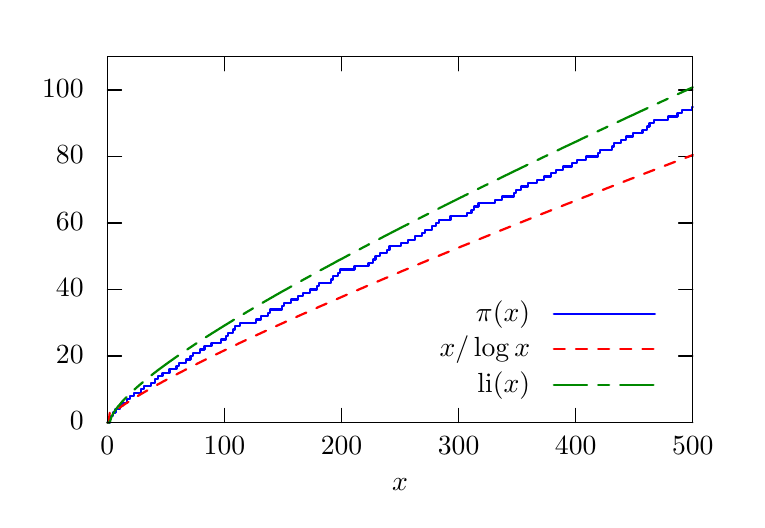
\begin{tikzpicture}[gnuplot]
%% generated with GNUPLOT 5.1p0 (Lua 5.3; terminal rev. 99, script rev. 100)
%% 木 11/22 15:28:55 2018
\path (0.000,0.000) rectangle (9.000,6.000);
\gpcolor{color=gp lt color border}
\gpsetlinetype{gp lt border}
\gpsetdashtype{gp dt solid}
\gpsetlinewidth{1.00}
\draw[gp path] (1.012,0.985)--(1.192,0.985);
\draw[gp path] (8.447,0.985)--(8.267,0.985);
\node[gp node right] at (0.828,0.985) {$0$};
\draw[gp path] (1.012,1.830)--(1.192,1.830);
\draw[gp path] (8.447,1.830)--(8.267,1.830);
\node[gp node right] at (0.828,1.830) {$20$};
\draw[gp path] (1.012,2.674)--(1.192,2.674);
\draw[gp path] (8.447,2.674)--(8.267,2.674);
\node[gp node right] at (0.828,2.674) {$40$};
\draw[gp path] (1.012,3.519)--(1.192,3.519);
\draw[gp path] (8.447,3.519)--(8.267,3.519);
\node[gp node right] at (0.828,3.519) {$60$};
\draw[gp path] (1.012,4.364)--(1.192,4.364);
\draw[gp path] (8.447,4.364)--(8.267,4.364);
\node[gp node right] at (0.828,4.364) {$80$};
\draw[gp path] (1.012,5.209)--(1.192,5.209);
\draw[gp path] (8.447,5.209)--(8.267,5.209);
\node[gp node right] at (0.828,5.209) {$100$};
\draw[gp path] (1.012,0.985)--(1.012,1.165);
\draw[gp path] (1.012,5.631)--(1.012,5.451);
\node[gp node center] at (1.012,0.677) {$0$};
\draw[gp path] (2.499,0.985)--(2.499,1.165);
\draw[gp path] (2.499,5.631)--(2.499,5.451);
\node[gp node center] at (2.499,0.677) {$100$};
\draw[gp path] (3.986,0.985)--(3.986,1.165);
\draw[gp path] (3.986,5.631)--(3.986,5.451);
\node[gp node center] at (3.986,0.677) {$200$};
\draw[gp path] (5.473,0.985)--(5.473,1.165);
\draw[gp path] (5.473,5.631)--(5.473,5.451);
\node[gp node center] at (5.473,0.677) {$300$};
\draw[gp path] (6.960,0.985)--(6.960,1.165);
\draw[gp path] (6.960,5.631)--(6.960,5.451);
\node[gp node center] at (6.960,0.677) {$400$};
\draw[gp path] (8.447,0.985)--(8.447,1.165);
\draw[gp path] (8.447,5.631)--(8.447,5.451);
\node[gp node center] at (8.447,0.677) {$500$};
\draw[gp path] (1.012,5.631)--(1.012,0.985)--(8.447,0.985)--(8.447,5.631)--cycle;
\node[gp node center] at (4.729,0.215) {$x$};
\node[gp node right] at (6.498,2.365) {$\pi(x)$};
\gpcolor{rgb color={0.000,0.000,1.000}}
\gpsetlinewidth{2.00}
\draw[gp path] (6.682,2.365)--(7.966,2.365);
\draw[gp path] (1.012,0.985)--(1.027,0.985)--(1.042,0.985)--(1.042,1.027)--(1.057,1.027)%
  --(1.057,1.069)--(1.071,1.069)--(1.086,1.069)--(1.086,1.112)--(1.101,1.112)--(1.116,1.112)%
  --(1.116,1.154)--(1.131,1.154)--(1.146,1.154)--(1.161,1.154)--(1.176,1.154)--(1.176,1.196)%
  --(1.190,1.196)--(1.205,1.196)--(1.205,1.238)--(1.220,1.238)--(1.235,1.238)--(1.250,1.238)%
  --(1.265,1.238)--(1.265,1.281)--(1.280,1.281)--(1.295,1.281)--(1.295,1.323)--(1.309,1.323)%
  --(1.324,1.323)--(1.339,1.323)--(1.354,1.323)--(1.354,1.365)--(1.369,1.365)--(1.384,1.365)%
  --(1.399,1.365)--(1.413,1.365)--(1.428,1.365)--(1.443,1.365)--(1.443,1.407)--(1.458,1.407)%
  --(1.473,1.407)--(1.473,1.450)--(1.488,1.450)--(1.503,1.450)--(1.518,1.450)--(1.532,1.450)%
  --(1.547,1.450)--(1.562,1.450)--(1.562,1.492)--(1.577,1.492)--(1.592,1.492)--(1.607,1.492)%
  --(1.622,1.492)--(1.622,1.534)--(1.637,1.534)--(1.651,1.534)--(1.651,1.576)--(1.666,1.576)%
  --(1.681,1.576)--(1.696,1.576)--(1.711,1.576)--(1.711,1.619)--(1.726,1.619)--(1.741,1.619)%
  --(1.756,1.619)--(1.770,1.619)--(1.785,1.619)--(1.800,1.619)--(1.800,1.661)--(1.815,1.661)%
  --(1.830,1.661)--(1.845,1.661)--(1.860,1.661)--(1.874,1.661)--(1.889,1.661)--(1.889,1.703)%
  --(1.904,1.703)--(1.919,1.703)--(1.919,1.745)--(1.934,1.745)--(1.949,1.745)--(1.964,1.745)%
  --(1.979,1.745)--(1.993,1.745)--(2.008,1.745)--(2.008,1.787)--(2.023,1.787)--(2.038,1.787)%
  --(2.053,1.787)--(2.068,1.787)--(2.068,1.830)--(2.083,1.830)--(2.098,1.830)--(2.098,1.872)%
  --(2.112,1.872)--(2.127,1.872)--(2.142,1.872)--(2.157,1.872)--(2.172,1.872)--(2.187,1.872)%
  --(2.187,1.914)--(2.202,1.914)--(2.216,1.914)--(2.231,1.914)--(2.246,1.914)--(2.246,1.956)%
  --(2.261,1.956)--(2.276,1.956)--(2.291,1.956)--(2.306,1.956)--(2.321,1.956)--(2.335,1.956)%
  --(2.335,1.999)--(2.350,1.999)--(2.365,1.999)--(2.380,1.999)--(2.395,1.999)--(2.410,1.999)%
  --(2.425,1.999)--(2.440,1.999)--(2.454,1.999)--(2.454,2.041)--(2.469,2.041)--(2.484,2.041)%
  --(2.499,2.041)--(2.514,2.041)--(2.514,2.083)--(2.529,2.083)--(2.544,2.083)--(2.544,2.125)%
  --(2.558,2.125)--(2.573,2.125)--(2.588,2.125)--(2.603,2.125)--(2.603,2.168)--(2.618,2.168)%
  --(2.633,2.168)--(2.633,2.210)--(2.648,2.210)--(2.663,2.210)--(2.677,2.210)--(2.692,2.210)%
  --(2.692,2.252)--(2.707,2.252)--(2.722,2.252)--(2.737,2.252)--(2.752,2.252)--(2.767,2.252)%
  --(2.782,2.252)--(2.796,2.252)--(2.811,2.252)--(2.826,2.252)--(2.841,2.252)--(2.856,2.252)%
  --(2.871,2.252)--(2.886,2.252)--(2.900,2.252)--(2.900,2.294)--(2.915,2.294)--(2.930,2.294)%
  --(2.945,2.294)--(2.960,2.294)--(2.960,2.337)--(2.975,2.337)--(2.990,2.337)--(3.005,2.337)%
  --(3.019,2.337)--(3.034,2.337)--(3.049,2.337)--(3.049,2.379)--(3.064,2.379)--(3.079,2.379)%
  --(3.079,2.421)--(3.094,2.421)--(3.109,2.421)--(3.124,2.421)--(3.138,2.421)--(3.153,2.421)%
  --(3.168,2.421)--(3.183,2.421)--(3.198,2.421)--(3.213,2.421)--(3.228,2.421)--(3.228,2.463)%
  --(3.243,2.463)--(3.257,2.463)--(3.257,2.506)--(3.272,2.506)--(3.287,2.506)--(3.302,2.506)%
  --(3.317,2.506)--(3.332,2.506)--(3.347,2.506)--(3.347,2.548)--(3.361,2.548)--(3.376,2.548)%
  --(3.391,2.548)--(3.406,2.548)--(3.421,2.548)--(3.436,2.548)--(3.436,2.590)--(3.451,2.590)%
  --(3.466,2.590)--(3.480,2.590)--(3.495,2.590)--(3.495,2.632)--(3.510,2.632)--(3.525,2.632)%
  --(3.540,2.632)--(3.555,2.632)--(3.570,2.632)--(3.585,2.632)--(3.585,2.674)--(3.599,2.674)%
  --(3.614,2.674)--(3.629,2.674)--(3.644,2.674)--(3.659,2.674)--(3.674,2.674)--(3.674,2.717)%
  --(3.689,2.717)--(3.703,2.717)--(3.703,2.759)--(3.718,2.759)--(3.733,2.759)--(3.748,2.759)%
  --(3.763,2.759)--(3.778,2.759)--(3.793,2.759)--(3.808,2.759)--(3.822,2.759)--(3.837,2.759)%
  --(3.852,2.759)--(3.852,2.801)--(3.867,2.801)--(3.882,2.801)--(3.882,2.843)--(3.897,2.843)%
  --(3.912,2.843)--(3.927,2.843)--(3.941,2.843)--(3.941,2.886)--(3.956,2.886)--(3.971,2.886)%
  --(3.971,2.928)--(3.986,2.928)--(4.001,2.928)--(4.016,2.928)--(4.031,2.928)--(4.045,2.928)%
  --(4.060,2.928)--(4.075,2.928)--(4.090,2.928)--(4.105,2.928)--(4.120,2.928)--(4.135,2.928)%
  --(4.150,2.928)--(4.150,2.970)--(4.164,2.970)--(4.179,2.970)--(4.194,2.970)--(4.209,2.970)%
  --(4.224,2.970)--(4.239,2.970)--(4.254,2.970)--(4.269,2.970)--(4.283,2.970)--(4.298,2.970)%
  --(4.313,2.970)--(4.328,2.970)--(4.328,3.012)--(4.343,3.012)--(4.358,3.012)--(4.373,3.012)%
  --(4.387,3.012)--(4.387,3.055)--(4.402,3.055)--(4.417,3.055)--(4.417,3.097)--(4.432,3.097)%
  --(4.447,3.097)--(4.462,3.097)--(4.477,3.097)--(4.477,3.139)--(4.492,3.139)--(4.506,3.139)%
  --(4.521,3.139)--(4.536,3.139)--(4.551,3.139)--(4.566,3.139)--(4.566,3.181)--(4.581,3.181)%
  --(4.596,3.181)--(4.596,3.224)--(4.611,3.224)--(4.625,3.224)--(4.640,3.224)--(4.655,3.224)%
  --(4.670,3.224)--(4.685,3.224)--(4.700,3.224)--(4.715,3.224)--(4.730,3.224)--(4.744,3.224)%
  --(4.744,3.266)--(4.759,3.266)--(4.774,3.266)--(4.789,3.266)--(4.804,3.266)--(4.819,3.266)%
  --(4.834,3.266)--(4.834,3.308)--(4.848,3.308)--(4.863,3.308)--(4.878,3.308)--(4.893,3.308)%
  --(4.908,3.308)--(4.923,3.308)--(4.923,3.350)--(4.938,3.350)--(4.953,3.350)--(4.967,3.350)%
  --(4.982,3.350)--(4.997,3.350)--(5.012,3.350)--(5.012,3.392)--(5.027,3.392)--(5.042,3.392)%
  --(5.042,3.435)--(5.057,3.435)--(5.072,3.435)--(5.086,3.435)--(5.101,3.435)--(5.116,3.435)%
  --(5.131,3.435)--(5.131,3.477)--(5.146,3.477)--(5.161,3.477)--(5.176,3.477)--(5.190,3.477)%
  --(5.190,3.519)--(5.205,3.519)--(5.220,3.519)--(5.220,3.561)--(5.235,3.561)--(5.250,3.561)%
  --(5.265,3.561)--(5.280,3.561)--(5.295,3.561)--(5.309,3.561)--(5.324,3.561)--(5.339,3.561)%
  --(5.354,3.561)--(5.369,3.561)--(5.369,3.604)--(5.384,3.604)--(5.399,3.604)--(5.414,3.604)%
  --(5.428,3.604)--(5.443,3.604)--(5.458,3.604)--(5.473,3.604)--(5.488,3.604)--(5.503,3.604)%
  --(5.518,3.604)--(5.532,3.604)--(5.547,3.604)--(5.562,3.604)--(5.577,3.604)--(5.577,3.646)%
  --(5.592,3.646)--(5.607,3.646)--(5.622,3.646)--(5.637,3.646)--(5.637,3.688)--(5.651,3.688)%
  --(5.666,3.688)--(5.666,3.730)--(5.681,3.730)--(5.696,3.730)--(5.711,3.730)--(5.726,3.730)%
  --(5.726,3.773)--(5.741,3.773)--(5.756,3.773)--(5.770,3.773)--(5.785,3.773)--(5.800,3.773)%
  --(5.815,3.773)--(5.830,3.773)--(5.845,3.773)--(5.860,3.773)--(5.874,3.773)--(5.889,3.773)%
  --(5.904,3.773)--(5.919,3.773)--(5.934,3.773)--(5.934,3.815)--(5.949,3.815)--(5.964,3.815)%
  --(5.979,3.815)--(5.993,3.815)--(6.008,3.815)--(6.023,3.815)--(6.023,3.857)--(6.038,3.857)%
  --(6.053,3.857)--(6.068,3.857)--(6.083,3.857)--(6.098,3.857)--(6.112,3.857)--(6.127,3.857)%
  --(6.142,3.857)--(6.157,3.857)--(6.172,3.857)--(6.172,3.899)--(6.187,3.899)--(6.202,3.899)%
  --(6.202,3.942)--(6.217,3.942)--(6.231,3.942)--(6.246,3.942)--(6.261,3.942)--(6.261,3.984)%
  --(6.276,3.984)--(6.291,3.984)--(6.306,3.984)--(6.321,3.984)--(6.335,3.984)--(6.350,3.984)%
  --(6.350,4.026)--(6.365,4.026)--(6.380,4.026)--(6.395,4.026)--(6.410,4.026)--(6.425,4.026)%
  --(6.440,4.026)--(6.454,4.026)--(6.469,4.026)--(6.469,4.068)--(6.484,4.068)--(6.499,4.068)%
  --(6.514,4.068)--(6.529,4.068)--(6.544,4.068)--(6.559,4.068)--(6.559,4.110)--(6.573,4.110)%
  --(6.588,4.110)--(6.603,4.110)--(6.618,4.110)--(6.633,4.110)--(6.648,4.110)--(6.648,4.153)%
  --(6.663,4.153)--(6.677,4.153)--(6.692,4.153)--(6.707,4.153)--(6.707,4.195)--(6.722,4.195)%
  --(6.737,4.195)--(6.752,4.195)--(6.767,4.195)--(6.782,4.195)--(6.796,4.195)--(6.796,4.237)%
  --(6.811,4.237)--(6.826,4.237)--(6.841,4.237)--(6.856,4.237)--(6.871,4.237)--(6.886,4.237)%
  --(6.901,4.237)--(6.915,4.237)--(6.915,4.279)--(6.930,4.279)--(6.945,4.279)--(6.960,4.279)%
  --(6.975,4.279)--(6.975,4.322)--(6.990,4.322)--(7.005,4.322)--(7.019,4.322)--(7.034,4.322)%
  --(7.049,4.322)--(7.064,4.322)--(7.079,4.322)--(7.094,4.322)--(7.094,4.364)--(7.109,4.364)%
  --(7.124,4.364)--(7.138,4.364)--(7.153,4.364)--(7.168,4.364)--(7.183,4.364)--(7.198,4.364)%
  --(7.213,4.364)--(7.228,4.364)--(7.243,4.364)--(7.243,4.406)--(7.257,4.406)--(7.272,4.406)%
  --(7.272,4.448)--(7.287,4.448)--(7.302,4.448)--(7.317,4.448)--(7.332,4.448)--(7.347,4.448)%
  --(7.361,4.448)--(7.376,4.448)--(7.391,4.448)--(7.406,4.448)--(7.421,4.448)--(7.421,4.491)%
  --(7.436,4.491)--(7.451,4.491)--(7.451,4.533)--(7.466,4.533)--(7.480,4.533)--(7.495,4.533)%
  --(7.510,4.533)--(7.525,4.533)--(7.540,4.533)--(7.540,4.575)--(7.555,4.575)--(7.570,4.575)%
  --(7.585,4.575)--(7.599,4.575)--(7.599,4.617)--(7.614,4.617)--(7.629,4.617)--(7.644,4.617)%
  --(7.659,4.617)--(7.674,4.617)--(7.689,4.617)--(7.689,4.660)--(7.704,4.660)--(7.718,4.660)%
  --(7.733,4.660)--(7.748,4.660)--(7.763,4.660)--(7.778,4.660)--(7.793,4.660)--(7.808,4.660)%
  --(7.808,4.702)--(7.822,4.702)--(7.837,4.702)--(7.852,4.702)--(7.867,4.702)--(7.867,4.744)%
  --(7.882,4.744)--(7.897,4.744)--(7.897,4.786)--(7.912,4.786)--(7.927,4.786)--(7.941,4.786)%
  --(7.956,4.786)--(7.956,4.829)--(7.971,4.829)--(7.986,4.829)--(8.001,4.829)--(8.016,4.829)%
  --(8.031,4.829)--(8.046,4.829)--(8.060,4.829)--(8.075,4.829)--(8.090,4.829)--(8.105,4.829)%
  --(8.120,4.829)--(8.135,4.829)--(8.135,4.871)--(8.150,4.871)--(8.164,4.871)--(8.179,4.871)%
  --(8.194,4.871)--(8.209,4.871)--(8.224,4.871)--(8.239,4.871)--(8.254,4.871)--(8.254,4.913)%
  --(8.269,4.913)--(8.283,4.913)--(8.298,4.913)--(8.313,4.913)--(8.313,4.955)--(8.328,4.955)%
  --(8.343,4.955)--(8.358,4.955)--(8.373,4.955)--(8.388,4.955)--(8.402,4.955)--(8.417,4.955)%
  --(8.432,4.955)--(8.432,4.997)--(8.447,4.997);
\gpcolor{color=gp lt color border}
\node[gp node right] at (6.498,1.915) {$x/\log x$};
\gpcolor{rgb color={1.000,0.000,0.000}}
\gpsetdashtype{dash pattern=on 5.00*\gpdashlength off 5.00*\gpdashlength }
\draw[gp path] (6.682,1.915)--(7.966,1.915);
\draw[gp path] (1.012,0.985)--(1.027,0.985)--(1.042,1.107)--(1.057,1.100)--(1.071,1.107)%
  --(1.086,1.116)--(1.101,1.126)--(1.116,1.137)--(1.131,1.147)--(1.146,1.158)--(1.161,1.168)%
  --(1.176,1.179)--(1.190,1.189)--(1.205,1.199)--(1.220,1.209)--(1.235,1.219)--(1.250,1.229)%
  --(1.265,1.238)--(1.280,1.248)--(1.295,1.258)--(1.309,1.267)--(1.324,1.276)--(1.339,1.286)%
  --(1.354,1.295)--(1.369,1.304)--(1.384,1.313)--(1.399,1.322)--(1.413,1.331)--(1.428,1.340)%
  --(1.443,1.349)--(1.458,1.358)--(1.473,1.366)--(1.488,1.375)--(1.503,1.384)--(1.518,1.392)%
  --(1.532,1.401)--(1.547,1.409)--(1.562,1.418)--(1.577,1.426)--(1.592,1.435)--(1.607,1.443)%
  --(1.622,1.451)--(1.637,1.460)--(1.651,1.468)--(1.666,1.476)--(1.681,1.484)--(1.696,1.492)%
  --(1.711,1.501)--(1.726,1.509)--(1.741,1.517)--(1.756,1.525)--(1.770,1.533)--(1.785,1.541)%
  --(1.800,1.549)--(1.815,1.557)--(1.830,1.565)--(1.845,1.573)--(1.860,1.580)--(1.874,1.588)%
  --(1.889,1.596)--(1.904,1.604)--(1.919,1.612)--(1.934,1.619)--(1.949,1.627)--(1.964,1.635)%
  --(1.979,1.643)--(1.993,1.650)--(2.008,1.658)--(2.023,1.666)--(2.038,1.673)--(2.053,1.681)%
  --(2.068,1.688)--(2.083,1.696)--(2.098,1.704)--(2.112,1.711)--(2.127,1.719)--(2.142,1.726)%
  --(2.157,1.734)--(2.172,1.741)--(2.187,1.749)--(2.202,1.756)--(2.216,1.764)--(2.231,1.771)%
  --(2.246,1.778)--(2.261,1.786)--(2.276,1.793)--(2.291,1.800)--(2.306,1.808)--(2.321,1.815)%
  --(2.335,1.822)--(2.350,1.830)--(2.365,1.837)--(2.380,1.844)--(2.395,1.852)--(2.410,1.859)%
  --(2.425,1.866)--(2.440,1.873)--(2.454,1.881)--(2.469,1.888)--(2.484,1.895)--(2.499,1.902)%
  --(2.514,1.909)--(2.529,1.916)--(2.544,1.924)--(2.558,1.931)--(2.573,1.938)--(2.588,1.945)%
  --(2.603,1.952)--(2.618,1.959)--(2.633,1.966)--(2.648,1.973)--(2.663,1.980)--(2.677,1.988)%
  --(2.692,1.995)--(2.707,2.002)--(2.722,2.009)--(2.737,2.016)--(2.752,2.023)--(2.767,2.030)%
  --(2.782,2.037)--(2.796,2.044)--(2.811,2.051)--(2.826,2.058)--(2.841,2.065)--(2.856,2.072)%
  --(2.871,2.078)--(2.886,2.085)--(2.900,2.092)--(2.915,2.099)--(2.930,2.106)--(2.945,2.113)%
  --(2.960,2.120)--(2.975,2.127)--(2.990,2.134)--(3.005,2.141)--(3.019,2.147)--(3.034,2.154)%
  --(3.049,2.161)--(3.064,2.168)--(3.079,2.175)--(3.094,2.182)--(3.109,2.188)--(3.124,2.195)%
  --(3.138,2.202)--(3.153,2.209)--(3.168,2.216)--(3.183,2.222)--(3.198,2.229)--(3.213,2.236)%
  --(3.228,2.243)--(3.243,2.249)--(3.257,2.256)--(3.272,2.263)--(3.287,2.270)--(3.302,2.276)%
  --(3.317,2.283)--(3.332,2.290)--(3.347,2.296)--(3.361,2.303)--(3.376,2.310)--(3.391,2.317)%
  --(3.406,2.323)--(3.421,2.330)--(3.436,2.337)--(3.451,2.343)--(3.466,2.350)--(3.480,2.357)%
  --(3.495,2.363)--(3.510,2.370)--(3.525,2.376)--(3.540,2.383)--(3.555,2.390)--(3.570,2.396)%
  --(3.585,2.403)--(3.599,2.410)--(3.614,2.416)--(3.629,2.423)--(3.644,2.429)--(3.659,2.436)%
  --(3.674,2.442)--(3.689,2.449)--(3.703,2.456)--(3.718,2.462)--(3.733,2.469)--(3.748,2.475)%
  --(3.763,2.482)--(3.778,2.488)--(3.793,2.495)--(3.808,2.501)--(3.822,2.508)--(3.837,2.514)%
  --(3.852,2.521)--(3.867,2.527)--(3.882,2.534)--(3.897,2.540)--(3.912,2.547)--(3.927,2.553)%
  --(3.941,2.560)--(3.956,2.566)--(3.971,2.573)--(3.986,2.579)--(4.001,2.586)--(4.016,2.592)%
  --(4.031,2.599)--(4.045,2.605)--(4.060,2.612)--(4.075,2.618)--(4.090,2.624)--(4.105,2.631)%
  --(4.120,2.637)--(4.135,2.644)--(4.150,2.650)--(4.164,2.657)--(4.179,2.663)--(4.194,2.669)%
  --(4.209,2.676)--(4.224,2.682)--(4.239,2.689)--(4.254,2.695)--(4.269,2.701)--(4.283,2.708)%
  --(4.298,2.714)--(4.313,2.721)--(4.328,2.727)--(4.343,2.733)--(4.358,2.740)--(4.373,2.746)%
  --(4.387,2.752)--(4.402,2.759)--(4.417,2.765)--(4.432,2.771)--(4.447,2.778)--(4.462,2.784)%
  --(4.477,2.790)--(4.492,2.797)--(4.506,2.803)--(4.521,2.809)--(4.536,2.816)--(4.551,2.822)%
  --(4.566,2.828)--(4.581,2.835)--(4.596,2.841)--(4.611,2.847)--(4.625,2.853)--(4.640,2.860)%
  --(4.655,2.866)--(4.670,2.872)--(4.685,2.879)--(4.700,2.885)--(4.715,2.891)--(4.730,2.897)%
  --(4.744,2.904)--(4.759,2.910)--(4.774,2.916)--(4.789,2.922)--(4.804,2.929)--(4.819,2.935)%
  --(4.834,2.941)--(4.848,2.947)--(4.863,2.954)--(4.878,2.960)--(4.893,2.966)--(4.908,2.972)%
  --(4.923,2.979)--(4.938,2.985)--(4.953,2.991)--(4.967,2.997)--(4.982,3.003)--(4.997,3.010)%
  --(5.012,3.016)--(5.027,3.022)--(5.042,3.028)--(5.057,3.034)--(5.072,3.041)--(5.086,3.047)%
  --(5.101,3.053)--(5.116,3.059)--(5.131,3.065)--(5.146,3.071)--(5.161,3.078)--(5.176,3.084)%
  --(5.190,3.090)--(5.205,3.096)--(5.220,3.102)--(5.235,3.108)--(5.250,3.115)--(5.265,3.121)%
  --(5.280,3.127)--(5.295,3.133)--(5.309,3.139)--(5.324,3.145)--(5.339,3.151)--(5.354,3.158)%
  --(5.369,3.164)--(5.384,3.170)--(5.399,3.176)--(5.414,3.182)--(5.428,3.188)--(5.443,3.194)%
  --(5.458,3.200)--(5.473,3.206)--(5.488,3.213)--(5.503,3.219)--(5.518,3.225)--(5.532,3.231)%
  --(5.547,3.237)--(5.562,3.243)--(5.577,3.249)--(5.592,3.255)--(5.607,3.261)--(5.622,3.267)%
  --(5.637,3.273)--(5.651,3.280)--(5.666,3.286)--(5.681,3.292)--(5.696,3.298)--(5.711,3.304)%
  --(5.726,3.310)--(5.741,3.316)--(5.756,3.322)--(5.770,3.328)--(5.785,3.334)--(5.800,3.340)%
  --(5.815,3.346)--(5.830,3.352)--(5.845,3.358)--(5.860,3.364)--(5.874,3.370)--(5.889,3.376)%
  --(5.904,3.382)--(5.919,3.388)--(5.934,3.395)--(5.949,3.401)--(5.964,3.407)--(5.979,3.413)%
  --(5.993,3.419)--(6.008,3.425)--(6.023,3.431)--(6.038,3.437)--(6.053,3.443)--(6.068,3.449)%
  --(6.083,3.455)--(6.098,3.461)--(6.112,3.467)--(6.127,3.473)--(6.142,3.479)--(6.157,3.485)%
  --(6.172,3.491)--(6.187,3.497)--(6.202,3.503)--(6.217,3.509)--(6.231,3.515)--(6.246,3.520)%
  --(6.261,3.526)--(6.276,3.532)--(6.291,3.538)--(6.306,3.544)--(6.321,3.550)--(6.335,3.556)%
  --(6.350,3.562)--(6.365,3.568)--(6.380,3.574)--(6.395,3.580)--(6.410,3.586)--(6.425,3.592)%
  --(6.440,3.598)--(6.454,3.604)--(6.469,3.610)--(6.484,3.616)--(6.499,3.622)--(6.514,3.628)%
  --(6.529,3.634)--(6.544,3.640)--(6.559,3.645)--(6.573,3.651)--(6.588,3.657)--(6.603,3.663)%
  --(6.618,3.669)--(6.633,3.675)--(6.648,3.681)--(6.663,3.687)--(6.677,3.693)--(6.692,3.699)%
  --(6.707,3.705)--(6.722,3.711)--(6.737,3.716)--(6.752,3.722)--(6.767,3.728)--(6.782,3.734)%
  --(6.796,3.740)--(6.811,3.746)--(6.826,3.752)--(6.841,3.758)--(6.856,3.764)--(6.871,3.769)%
  --(6.886,3.775)--(6.901,3.781)--(6.915,3.787)--(6.930,3.793)--(6.945,3.799)--(6.960,3.805)%
  --(6.975,3.811)--(6.990,3.817)--(7.005,3.822)--(7.019,3.828)--(7.034,3.834)--(7.049,3.840)%
  --(7.064,3.846)--(7.079,3.852)--(7.094,3.858)--(7.109,3.863)--(7.124,3.869)--(7.138,3.875)%
  --(7.153,3.881)--(7.168,3.887)--(7.183,3.893)--(7.198,3.898)--(7.213,3.904)--(7.228,3.910)%
  --(7.243,3.916)--(7.257,3.922)--(7.272,3.928)--(7.287,3.934)--(7.302,3.939)--(7.317,3.945)%
  --(7.332,3.951)--(7.347,3.957)--(7.361,3.963)--(7.376,3.968)--(7.391,3.974)--(7.406,3.980)%
  --(7.421,3.986)--(7.436,3.992)--(7.451,3.998)--(7.466,4.003)--(7.480,4.009)--(7.495,4.015)%
  --(7.510,4.021)--(7.525,4.027)--(7.540,4.032)--(7.555,4.038)--(7.570,4.044)--(7.585,4.050)%
  --(7.599,4.056)--(7.614,4.061)--(7.629,4.067)--(7.644,4.073)--(7.659,4.079)--(7.674,4.085)%
  --(7.689,4.090)--(7.704,4.096)--(7.718,4.102)--(7.733,4.108)--(7.748,4.113)--(7.763,4.119)%
  --(7.778,4.125)--(7.793,4.131)--(7.808,4.137)--(7.822,4.142)--(7.837,4.148)--(7.852,4.154)%
  --(7.867,4.160)--(7.882,4.165)--(7.897,4.171)--(7.912,4.177)--(7.927,4.183)--(7.941,4.188)%
  --(7.956,4.194)--(7.971,4.200)--(7.986,4.206)--(8.001,4.211)--(8.016,4.217)--(8.031,4.223)%
  --(8.046,4.229)--(8.060,4.234)--(8.075,4.240)--(8.090,4.246)--(8.105,4.252)--(8.120,4.257)%
  --(8.135,4.263)--(8.150,4.269)--(8.164,4.275)--(8.179,4.280)--(8.194,4.286)--(8.209,4.292)%
  --(8.224,4.297)--(8.239,4.303)--(8.254,4.309)--(8.269,4.315)--(8.283,4.320)--(8.298,4.326)%
  --(8.313,4.332)--(8.328,4.337)--(8.343,4.343)--(8.358,4.349)--(8.373,4.355)--(8.388,4.360)%
  --(8.402,4.366)--(8.417,4.372)--(8.432,4.377)--(8.447,4.383);
\gpcolor{color=gp lt color border}
\node[gp node right] at (6.498,1.465) {$\mathrm{li}(x)$};
\gpcolor{rgb color={0.000,0.533,0.000}}
\gpsetdashtype{dash pattern=on 15.00*\gpdashlength off 5.00*\gpdashlength on 5.00*\gpdashlength off 5.00*\gpdashlength }
\draw[gp path] (6.682,1.465)--(7.966,1.465);
\draw[gp path] (1.012,0.985)--(1.027,0.985)--(1.042,0.985)--(1.057,1.037)--(1.071,1.071)%
  --(1.086,1.099)--(1.101,1.123)--(1.116,1.146)--(1.131,1.167)--(1.146,1.187)--(1.161,1.203)%
  --(1.176,1.221)--(1.190,1.239)--(1.205,1.256)--(1.220,1.272)--(1.235,1.288)--(1.250,1.303)%
  --(1.265,1.318)--(1.280,1.333)--(1.295,1.347)--(1.309,1.362)--(1.324,1.376)--(1.339,1.389)%
  --(1.354,1.403)--(1.369,1.416)--(1.384,1.430)--(1.399,1.443)--(1.413,1.455)--(1.428,1.468)%
  --(1.443,1.481)--(1.458,1.493)--(1.473,1.506)--(1.488,1.518)--(1.503,1.530)--(1.518,1.542)%
  --(1.532,1.554)--(1.547,1.566)--(1.562,1.578)--(1.577,1.590)--(1.592,1.602)--(1.607,1.614)%
  --(1.622,1.625)--(1.637,1.636)--(1.651,1.648)--(1.666,1.659)--(1.681,1.670)--(1.696,1.681)%
  --(1.711,1.692)--(1.726,1.703)--(1.741,1.714)--(1.756,1.725)--(1.770,1.735)--(1.785,1.746)%
  --(1.800,1.757)--(1.815,1.767)--(1.830,1.778)--(1.845,1.788)--(1.860,1.799)--(1.874,1.809)%
  --(1.889,1.820)--(1.904,1.830)--(1.919,1.840)--(1.934,1.851)--(1.949,1.861)--(1.964,1.871)%
  --(1.979,1.881)--(1.993,1.891)--(2.008,1.901)--(2.023,1.911)--(2.038,1.921)--(2.053,1.931)%
  --(2.068,1.941)--(2.083,1.951)--(2.098,1.961)--(2.112,1.971)--(2.127,1.980)--(2.142,1.990)%
  --(2.157,2.000)--(2.172,2.010)--(2.187,2.019)--(2.202,2.029)--(2.216,2.039)--(2.231,2.048)%
  --(2.246,2.058)--(2.261,2.067)--(2.276,2.077)--(2.291,2.086)--(2.306,2.096)--(2.321,2.105)%
  --(2.335,2.115)--(2.350,2.124)--(2.365,2.133)--(2.380,2.143)--(2.395,2.152)--(2.410,2.161)%
  --(2.425,2.171)--(2.440,2.180)--(2.454,2.189)--(2.469,2.198)--(2.484,2.208)--(2.499,2.217)%
  --(2.514,2.226)--(2.529,2.235)--(2.544,2.244)--(2.558,2.253)--(2.573,2.262)--(2.588,2.271)%
  --(2.603,2.281)--(2.618,2.290)--(2.633,2.299)--(2.648,2.308)--(2.663,2.317)--(2.677,2.326)%
  --(2.692,2.334)--(2.707,2.343)--(2.722,2.352)--(2.737,2.361)--(2.752,2.370)--(2.767,2.379)%
  --(2.782,2.388)--(2.796,2.397)--(2.811,2.405)--(2.826,2.414)--(2.841,2.423)--(2.856,2.432)%
  --(2.871,2.441)--(2.886,2.449)--(2.900,2.458)--(2.915,2.467)--(2.930,2.475)--(2.945,2.484)%
  --(2.960,2.493)--(2.975,2.501)--(2.990,2.510)--(3.005,2.519)--(3.019,2.527)--(3.034,2.536)%
  --(3.049,2.544)--(3.064,2.553)--(3.079,2.562)--(3.094,2.570)--(3.109,2.579)--(3.124,2.587)%
  --(3.138,2.596)--(3.153,2.604)--(3.168,2.613)--(3.183,2.621)--(3.198,2.630)--(3.213,2.638)%
  --(3.228,2.647)--(3.243,2.655)--(3.257,2.663)--(3.272,2.671)--(3.287,2.679)--(3.302,2.688)%
  --(3.317,2.696)--(3.332,2.705)--(3.347,2.713)--(3.361,2.721)--(3.376,2.730)--(3.391,2.738)%
  --(3.406,2.746)--(3.421,2.755)--(3.436,2.763)--(3.451,2.771)--(3.466,2.779)--(3.480,2.788)%
  --(3.495,2.796)--(3.510,2.804)--(3.525,2.812)--(3.540,2.821)--(3.555,2.829)--(3.570,2.837)%
  --(3.585,2.845)--(3.599,2.853)--(3.614,2.862)--(3.629,2.870)--(3.644,2.878)--(3.659,2.886)%
  --(3.674,2.894)--(3.689,2.902)--(3.703,2.911)--(3.718,2.919)--(3.733,2.927)--(3.748,2.935)%
  --(3.763,2.943)--(3.778,2.951)--(3.793,2.959)--(3.808,2.967)--(3.822,2.975)--(3.837,2.983)%
  --(3.852,2.991)--(3.867,2.999)--(3.882,3.007)--(3.897,3.016)--(3.912,3.024)--(3.927,3.032)%
  --(3.941,3.040)--(3.956,3.048)--(3.971,3.056)--(3.986,3.063)--(4.001,3.071)--(4.016,3.079)%
  --(4.031,3.087)--(4.045,3.095)--(4.060,3.103)--(4.075,3.111)--(4.090,3.119)--(4.105,3.127)%
  --(4.120,3.135)--(4.135,3.143)--(4.150,3.151)--(4.164,3.159)--(4.179,3.166)--(4.194,3.174)%
  --(4.209,3.182)--(4.224,3.190)--(4.239,3.198)--(4.254,3.206)--(4.269,3.214)--(4.283,3.221)%
  --(4.298,3.229)--(4.313,3.237)--(4.328,3.245)--(4.343,3.253)--(4.358,3.261)--(4.373,3.268)%
  --(4.387,3.276)--(4.402,3.284)--(4.417,3.292)--(4.432,3.299)--(4.447,3.307)--(4.462,3.315)%
  --(4.477,3.323)--(4.492,3.330)--(4.506,3.338)--(4.521,3.346)--(4.536,3.354)--(4.551,3.361)%
  --(4.566,3.369)--(4.581,3.377)--(4.596,3.385)--(4.611,3.392)--(4.625,3.400)--(4.640,3.408)%
  --(4.655,3.415)--(4.670,3.423)--(4.685,3.431)--(4.700,3.438)--(4.715,3.446)--(4.730,3.454)%
  --(4.744,3.461)--(4.759,3.469)--(4.774,3.477)--(4.789,3.484)--(4.804,3.492)--(4.819,3.499)%
  --(4.834,3.507)--(4.848,3.515)--(4.863,3.522)--(4.878,3.530)--(4.893,3.537)--(4.908,3.545)%
  --(4.923,3.553)--(4.938,3.560)--(4.953,3.568)--(4.967,3.575)--(4.982,3.583)--(4.997,3.590)%
  --(5.012,3.598)--(5.027,3.606)--(5.042,3.613)--(5.057,3.621)--(5.072,3.628)--(5.086,3.636)%
  --(5.101,3.643)--(5.116,3.651)--(5.131,3.658)--(5.146,3.666)--(5.161,3.673)--(5.176,3.681)%
  --(5.190,3.688)--(5.205,3.696)--(5.220,3.703)--(5.235,3.711)--(5.250,3.718)--(5.265,3.726)%
  --(5.280,3.733)--(5.295,3.741)--(5.309,3.748)--(5.324,3.755)--(5.339,3.763)--(5.354,3.770)%
  --(5.369,3.778)--(5.384,3.785)--(5.399,3.793)--(5.414,3.800)--(5.428,3.807)--(5.443,3.815)%
  --(5.458,3.822)--(5.473,3.830)--(5.488,3.837)--(5.503,3.845)--(5.518,3.852)--(5.532,3.859)%
  --(5.547,3.867)--(5.562,3.874)--(5.577,3.881)--(5.592,3.889)--(5.607,3.896)--(5.622,3.904)%
  --(5.637,3.911)--(5.651,3.918)--(5.666,3.926)--(5.681,3.933)--(5.696,3.940)--(5.711,3.948)%
  --(5.726,3.955)--(5.741,3.962)--(5.756,3.970)--(5.770,3.977)--(5.785,3.984)--(5.800,3.992)%
  --(5.815,3.999)--(5.830,4.006)--(5.845,4.014)--(5.860,4.021)--(5.874,4.028)--(5.889,4.035)%
  --(5.904,4.043)--(5.919,4.050)--(5.934,4.057)--(5.949,4.065)--(5.964,4.072)--(5.979,4.079)%
  --(5.993,4.086)--(6.008,4.094)--(6.023,4.101)--(6.038,4.108)--(6.053,4.115)--(6.068,4.123)%
  --(6.083,4.130)--(6.098,4.137)--(6.112,4.144)--(6.127,4.152)--(6.142,4.159)--(6.157,4.166)%
  --(6.172,4.173)--(6.187,4.181)--(6.202,4.188)--(6.217,4.195)--(6.231,4.202)--(6.246,4.209)%
  --(6.261,4.217)--(6.276,4.224)--(6.291,4.231)--(6.306,4.238)--(6.321,4.245)--(6.335,4.253)%
  --(6.350,4.260)--(6.365,4.267)--(6.380,4.274)--(6.395,4.281)--(6.410,4.288)--(6.425,4.296)%
  --(6.440,4.303)--(6.454,4.310)--(6.469,4.317)--(6.484,4.324)--(6.499,4.331)--(6.514,4.338)%
  --(6.529,4.346)--(6.544,4.353)--(6.559,4.360)--(6.573,4.367)--(6.588,4.374)--(6.603,4.381)%
  --(6.618,4.388)--(6.633,4.396)--(6.648,4.403)--(6.663,4.410)--(6.677,4.417)--(6.692,4.424)%
  --(6.707,4.431)--(6.722,4.438)--(6.737,4.445)--(6.752,4.452)--(6.767,4.459)--(6.782,4.467)%
  --(6.796,4.474)--(6.811,4.481)--(6.826,4.488)--(6.841,4.495)--(6.856,4.502)--(6.871,4.509)%
  --(6.886,4.516)--(6.901,4.523)--(6.915,4.530)--(6.930,4.537)--(6.945,4.544)--(6.960,4.551)%
  --(6.975,4.558)--(6.990,4.565)--(7.005,4.572)--(7.019,4.579)--(7.034,4.587)--(7.049,4.594)%
  --(7.064,4.601)--(7.079,4.608)--(7.094,4.615)--(7.109,4.622)--(7.124,4.629)--(7.138,4.636)%
  --(7.153,4.643)--(7.168,4.650)--(7.183,4.657)--(7.198,4.664)--(7.213,4.671)--(7.228,4.678)%
  --(7.243,4.685)--(7.257,4.692)--(7.272,4.699)--(7.287,4.706)--(7.302,4.713)--(7.317,4.720)%
  --(7.332,4.727)--(7.347,4.734)--(7.361,4.741)--(7.376,4.748)--(7.391,4.755)--(7.406,4.762)%
  --(7.421,4.768)--(7.436,4.775)--(7.451,4.782)--(7.466,4.789)--(7.480,4.796)--(7.495,4.803)%
  --(7.510,4.810)--(7.525,4.817)--(7.540,4.824)--(7.555,4.831)--(7.570,4.838)--(7.585,4.845)%
  --(7.599,4.852)--(7.614,4.859)--(7.629,4.866)--(7.644,4.873)--(7.659,4.880)--(7.674,4.886)%
  --(7.689,4.893)--(7.704,4.900)--(7.718,4.907)--(7.733,4.914)--(7.748,4.921)--(7.763,4.928)%
  --(7.778,4.935)--(7.793,4.942)--(7.808,4.949)--(7.822,4.956)--(7.837,4.962)--(7.852,4.969)%
  --(7.867,4.976)--(7.882,4.983)--(7.897,4.990)--(7.912,4.997)--(7.927,5.004)--(7.941,5.011)%
  --(7.956,5.017)--(7.971,5.024)--(7.986,5.031)--(8.001,5.038)--(8.016,5.045)--(8.031,5.052)%
  --(8.046,5.059)--(8.060,5.066)--(8.075,5.072)--(8.090,5.079)--(8.105,5.086)--(8.120,5.093)%
  --(8.135,5.100)--(8.150,5.107)--(8.164,5.113)--(8.179,5.120)--(8.194,5.127)--(8.209,5.134)%
  --(8.224,5.141)--(8.239,5.148)--(8.254,5.154)--(8.269,5.161)--(8.283,5.168)--(8.298,5.175)%
  --(8.313,5.182)--(8.328,5.189)--(8.343,5.195)--(8.358,5.202)--(8.373,5.209)--(8.388,5.216)%
  --(8.402,5.223)--(8.417,5.229)--(8.432,5.236)--(8.447,5.243);
\gpcolor{color=gp lt color border}
\gpsetdashtype{gp dt solid}
\gpsetlinewidth{1.00}
\draw[gp path] (1.012,5.631)--(1.012,0.985)--(8.447,0.985)--(8.447,5.631)--cycle;
%% coordinates of the plot area
\gpdefrectangularnode{gp plot 1}{\pgfpoint{1.012cm}{0.985cm}}{\pgfpoint{8.447cm}{5.631cm}}
\end{tikzpicture}

%   \caption{$\pi(x)$とその近似式}
%   % \label{fig:00}
% \end{figure}

\end{document}